\documentclass[aspectratio=169]{beamer}
\usetheme{default}
\usecolortheme{dove}
\setbeamertemplate{navigation symbols}{}
\setbeamertemplate{footline}[frame number]

\usepackage{lmodern}
\usepackage{microtype}
\usepackage{amsmath,amssymb}

\setbeamertemplate{section page}{%
  \centering\vfill
  {\Large\bfseries\thesection.~\insertsection}\par
  \vfill
}

\setbeamertemplate{subsection page}{%
  \centering\vfill
  {\Large\bfseries\thesection.~\insertsection}\par\vspace{0.6em}
  {\large\thesection.\thesubsection~~\insertsubsection}\par
  \vfill
}

\title{Identifying Heterogeneity by Time Between Shocks}
\subtitle{Exploiting exogenous variation in cyclone arrival timing}
\date{}

\begin{document}

\begin{frame}\titlepage\end{frame}

\begin{frame}{Outline}\tableofcontents\end{frame}

% ==================================================================
\section{The Problem}
% ==================================================================
\begin{frame}\sectionpage\end{frame}

\subsection{Baseline and current specification}
\begin{frame}\subsectionpage\end{frame}

\begin{frame}{Baseline specification (context, no gap)}
Before introducing the gap interaction, the workhorse LP estimates the \emph{average} effect of a Cat~1+ shock (64 knots, $n=374$ events):
\[
  y_{i,t+h} - y_{i,t-1}
  \;=\; \beta(h)\,\mathrm{shock}_{it}
  \;+\; \gamma_h'X_{it} + \alpha_{ih}(t) + \delta_{th} + \varepsilon_{ith}
\]
where $\beta(h)$ is estimated non-parametrically via horizon dummies (one coefficient per $h \in \{0, 1, \ldots, H\}$),
$X_{it}$ = two lags of GDP growth and shock, $\alpha_{ih}(t)$ = country$\times h$ FE with linear + quadratic trends, $\delta_{th}$ = year$\times h$ FE. Same-continent sample (182 countries). SE clustered by country.

\medskip
\textbf{This is spec (0) in the empirical section.} It pins down the average IRF and serves as the reference against which gap-interacted specifications are compared.
\end{frame}

\begin{frame}{Baseline IRF (no gap interaction)}
\centering
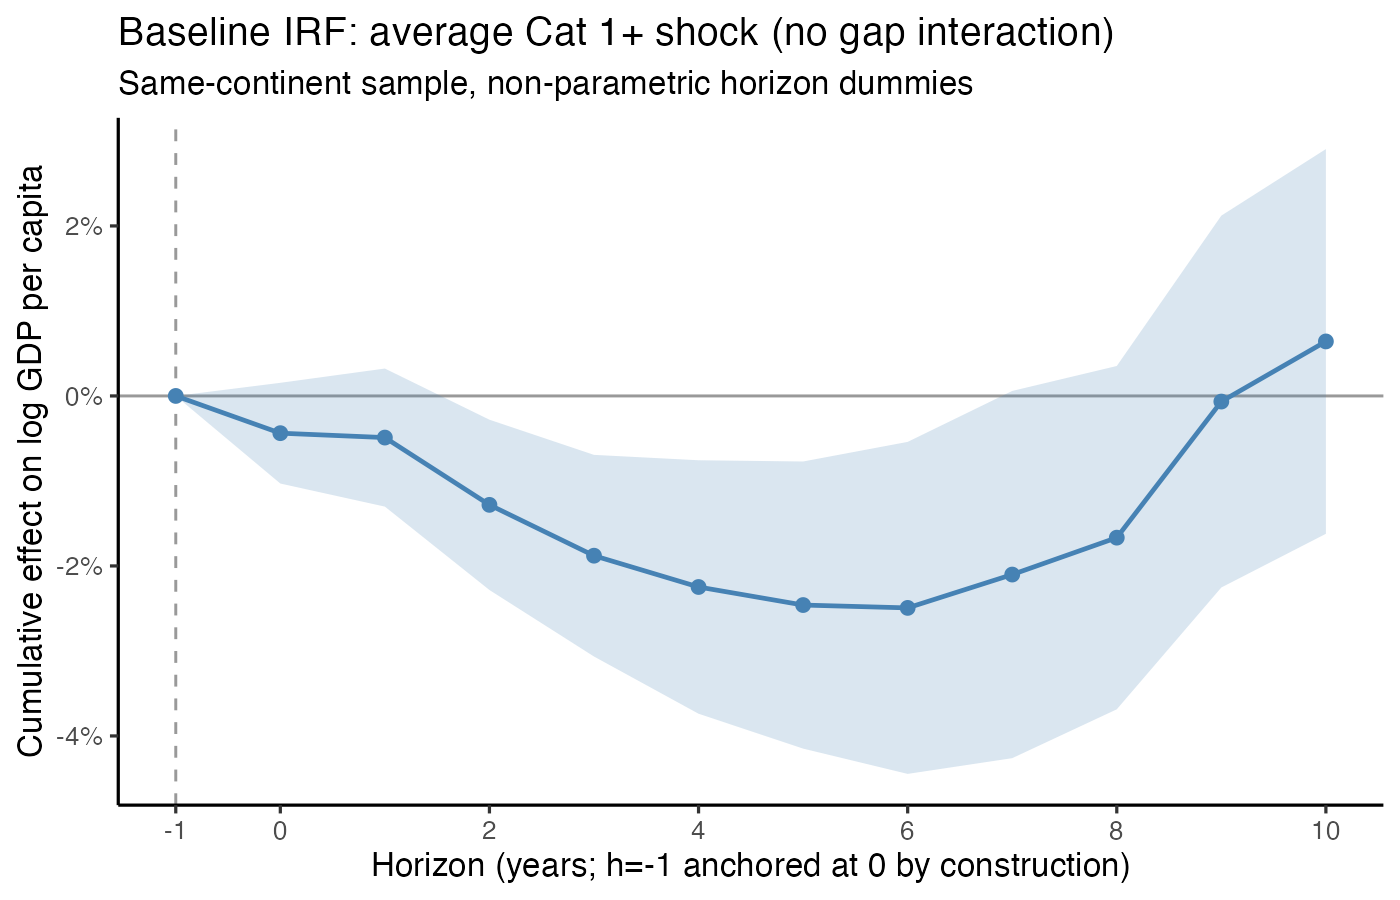
\includegraphics[width=0.78\textwidth,height=0.72\textheight,keepaspectratio]{figures/irf_baseline.png}

\smallskip
\small
Cumulative effect of a Cat~1+ shock on log GDP per capita, pooled across gap values. Reference curve for the gap-heterogeneity analysis.
\end{frame}

\begin{frame}{Current specification}
Stacked LP with continuous gap interaction, both $\beta(h)$ and $\phi(h)$ estimated \emph{non-parametrically} via horizon dummies:
\[
  y_{i,t+h} - y_{i,t-1}
  = \beta(h)\,\mathrm{shock}_{it}
  + \phi(h)\,\mathrm{shock}_{it}\times\mathrm{gap}_{it}
  + \gamma_h'X_{it} + \alpha_{ih}(t) + \delta_{th} + \varepsilon_{ith}
\]
where $\mathrm{gap}_{it}$ = years since country $i$'s previous Cat~1+ shock. One coefficient per horizon for each of $\beta$ and $\phi$; no polynomial restriction.

\medskip
\textbf{Finding:} compound shocks (short gap) less damaging than isolated shocks.

\medskip
\textbf{Question:} is $\phi(h)$ \emph{causally} identified?
\end{frame}

\subsection{Formal decomposition of the bias}
\begin{frame}\subsectionpage\end{frame}

\begin{frame}{Decomposing gap into between- and within-country}
Under a Poisson arrival model with rate $\lambda_i$:
\[
  \mathrm{gap}_{it} \;=\; \underbrace{1/\lambda_i}_{\text{between}} \;+\; \underbrace{\eta_{it}}_{\text{within (Poisson noise)}},
  \qquad \mathbb{E}[\eta_{it}\mid\lambda_i]=0.
\]
Only the within component is exogenous; the between component is confounded with country type.

\medskip
Under heterogeneous responses $\beta_i(h)=\bar\beta(h)+b(\lambda_i;h)+\nu_i$, the current spec has
\[
  \hat\phi(h)\;\xrightarrow{p}\;\phi_{\text{true}}(h)\;+\;\text{Cov}\!\big(1/\lambda_i,\,b(\lambda_i;h)\big)/\text{Var}(\cdot).
\]
If high-$\lambda$ countries adapt ($b'<0$), the bias is \emph{negative} --- exactly the compound-less-damaging gradient.
\end{frame}

\begin{frame}{Three channels of contamination}
\begin{enumerate}
  \item \textbf{Cross-country slope heterogeneity.} $\text{Cov}(1/\lambda_i,\beta_i)\neq 0$. Not absorbed by country FE on levels.

  \medskip
  \item \textbf{Sample selection on shock-years.} Long realized gaps occur during long uninterrupted stretches, so $\mathrm{gap}_{it}$ correlates with pre-period state even within country.

  \medskip
  \item \textbf{State-dependence of $\beta$.} If $\beta_i(h)$ depends on $y_{i,t-1}$, gap loads on state dependence rather than a causal timing effect.
\end{enumerate}

\medskip
Strategy~1 targets channel~1 only. Channels 2--3 motivate Strategies 2--3.
\end{frame}

% ==================================================================
\section{Strategy 1 --- Hazard Residualization}
% ==================================================================
\begin{frame}\sectionpage\end{frame}

\subsection{Method}
\begin{frame}\subsectionpage\end{frame}

\begin{frame}{Strategy 1: residualize gap against climatological hazard}
\textbf{Step 1.} Estimate each country's cyclone hazard rate. Simplest implementation (used here):
\[
  \hat\lambda_i \;=\; \frac{\#\ \text{Cat 1+ shock-years in country } i}{\#\ \text{years observed}}.
\]
More refined variants use the full IBTrACS track data (all storms passing within a radius of the centroid) and allow a smooth time trend $\hat\lambda_i(t)$ for climate change --- left for future work.

\medskip
\textbf{Step 2.} Define the surprise gap
\[
  \tilde{\mathrm{gap}}_{it} \;=\; \mathrm{gap}_{it} - \mathbb{E}[\mathrm{gap}\mid \hat\lambda_i(t)].
\]

\medskip
\textbf{Step 3.} Replace $\mathrm{shock}\times\mathrm{gap}$ with $\mathrm{shock}\times\tilde{\mathrm{gap}}$ in the LP.

\medskip
Mean-zero within country, orthogonal to hazard by construction.
\end{frame}

\begin{frame}{Strategy 1: a lazier variant}
Keep realized gap on the RHS but add $\mathrm{shock}\times\hat\lambda_i$ as an extra control:
\[
  \ldots + \phi(h)\,\mathrm{shock}\times\mathrm{gap}
         + \psi(h)\,\mathrm{shock}\times\hat\lambda_i + \ldots
\]

\medskip
Then $\phi(h)$ is identified from within-hazard variation only.

\medskip
\textbf{Role:} sanity check / cheapest first pass. If the compound$\to$isolated gradient survives residualization against $\hat\lambda_i$, cross-country contamination is not driving it.
\end{frame}

\subsection{Empirical results}
\begin{frame}\subsectionpage\end{frame}

\begin{frame}{Specifications estimated}
\footnotesize
Same-continent sample (182 countries, 374 Cat~1+ shocks). Stacked LP with non-parametric horizon dummies for both $\beta(h)$ and $\phi(h)$, clustered by country.

\smallskip
\begin{tabular}{l l l l}
\hline
\textbf{Spec} & \textbf{Interaction} & \textbf{Extra} & \textbf{FE} \\
\hline
(0) Baseline (no gap)     & \emph{none}                   &                        & country$\times h$ trends, year$\times h$ \\
(1) Replication           & shock $\times$ gap            &                        & country$\times h$ trends, year$\times h$ \\
(2) Residualized          & shock $\times$ gap\_resid     &                        & country$\times h$ trends, year$\times h$ \\
(3) Control for $1/\hat\lambda_i$ & shock $\times$ gap            & shock $\times\,1/\hat\lambda_i$ & country$\times h$ trends, year$\times h$ \\
(4) Region$\times$year    & shock $\times$ gap\_resid     &                        & country$\times h$ trends, \textbf{region$\times$year} \\
\hline
\end{tabular}

\medskip
$\text{gap\_resid}_{it} = \text{gap}_{it} - 1/\hat\lambda_i$ with $\hat\lambda_i$ = realized Cat~1+ rate.
\end{frame}

\begin{frame}{Diagnostic: gap variance decomposition}
Among shock-years only:
\[
  \mathrm{Var}(\mathrm{gap}_{it}) = 23.5, \qquad
  \underbrace{\mathrm{Var}_{\text{within}}}_{8.4\ (35.7\%)} \;+\; \underbrace{\mathrm{Var}_{\text{between}}}_{15.1\ (64.3\%)}
\]

\medskip
\textbf{Almost two-thirds} of the identifying variation in the current spec is cross-country. Under the formal decomposition, this is exactly the component confounded with $\lambda_i$.

\medskip
Residualization throws away the between share and keeps only the 35.7\% within-country Poisson-noise component. (At Cat~1+ the between share is even larger than at Cat~2+ because more countries are treated and the hazard rate spreads further.)
\end{frame}

\begin{frame}{Cross-country confound: gap vs.\ $1/\hat\lambda_i$}
\centering
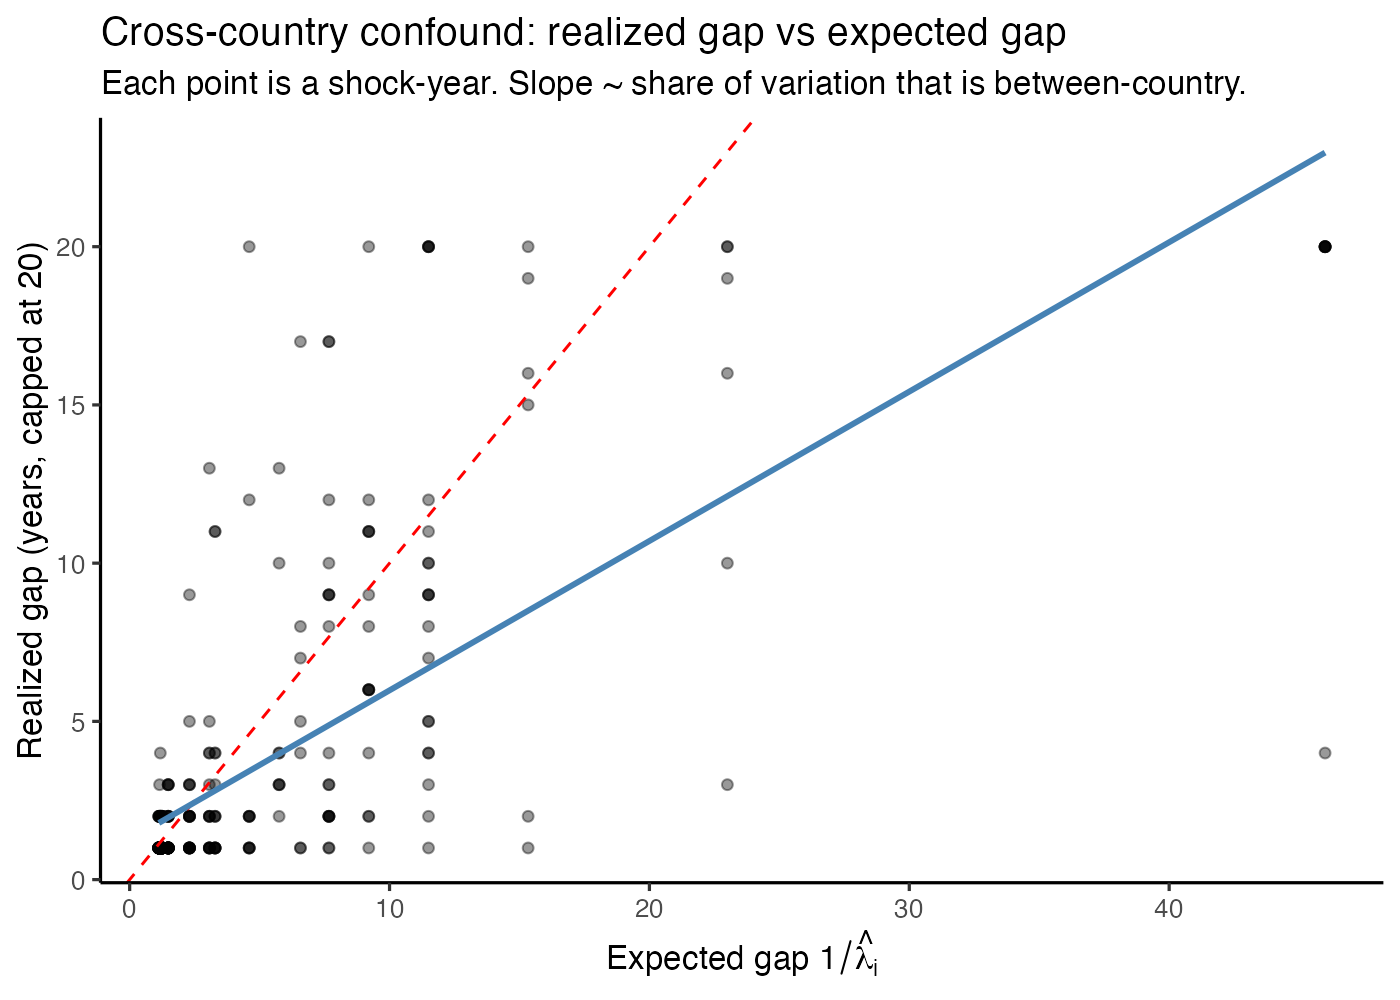
\includegraphics[width=0.72\textwidth,height=0.70\textheight,keepaspectratio]{figures/gap_vs_hazard.png}
\end{frame}

\begin{frame}{IRFs under the four specifications}
\centering
\makebox[\linewidth][c]{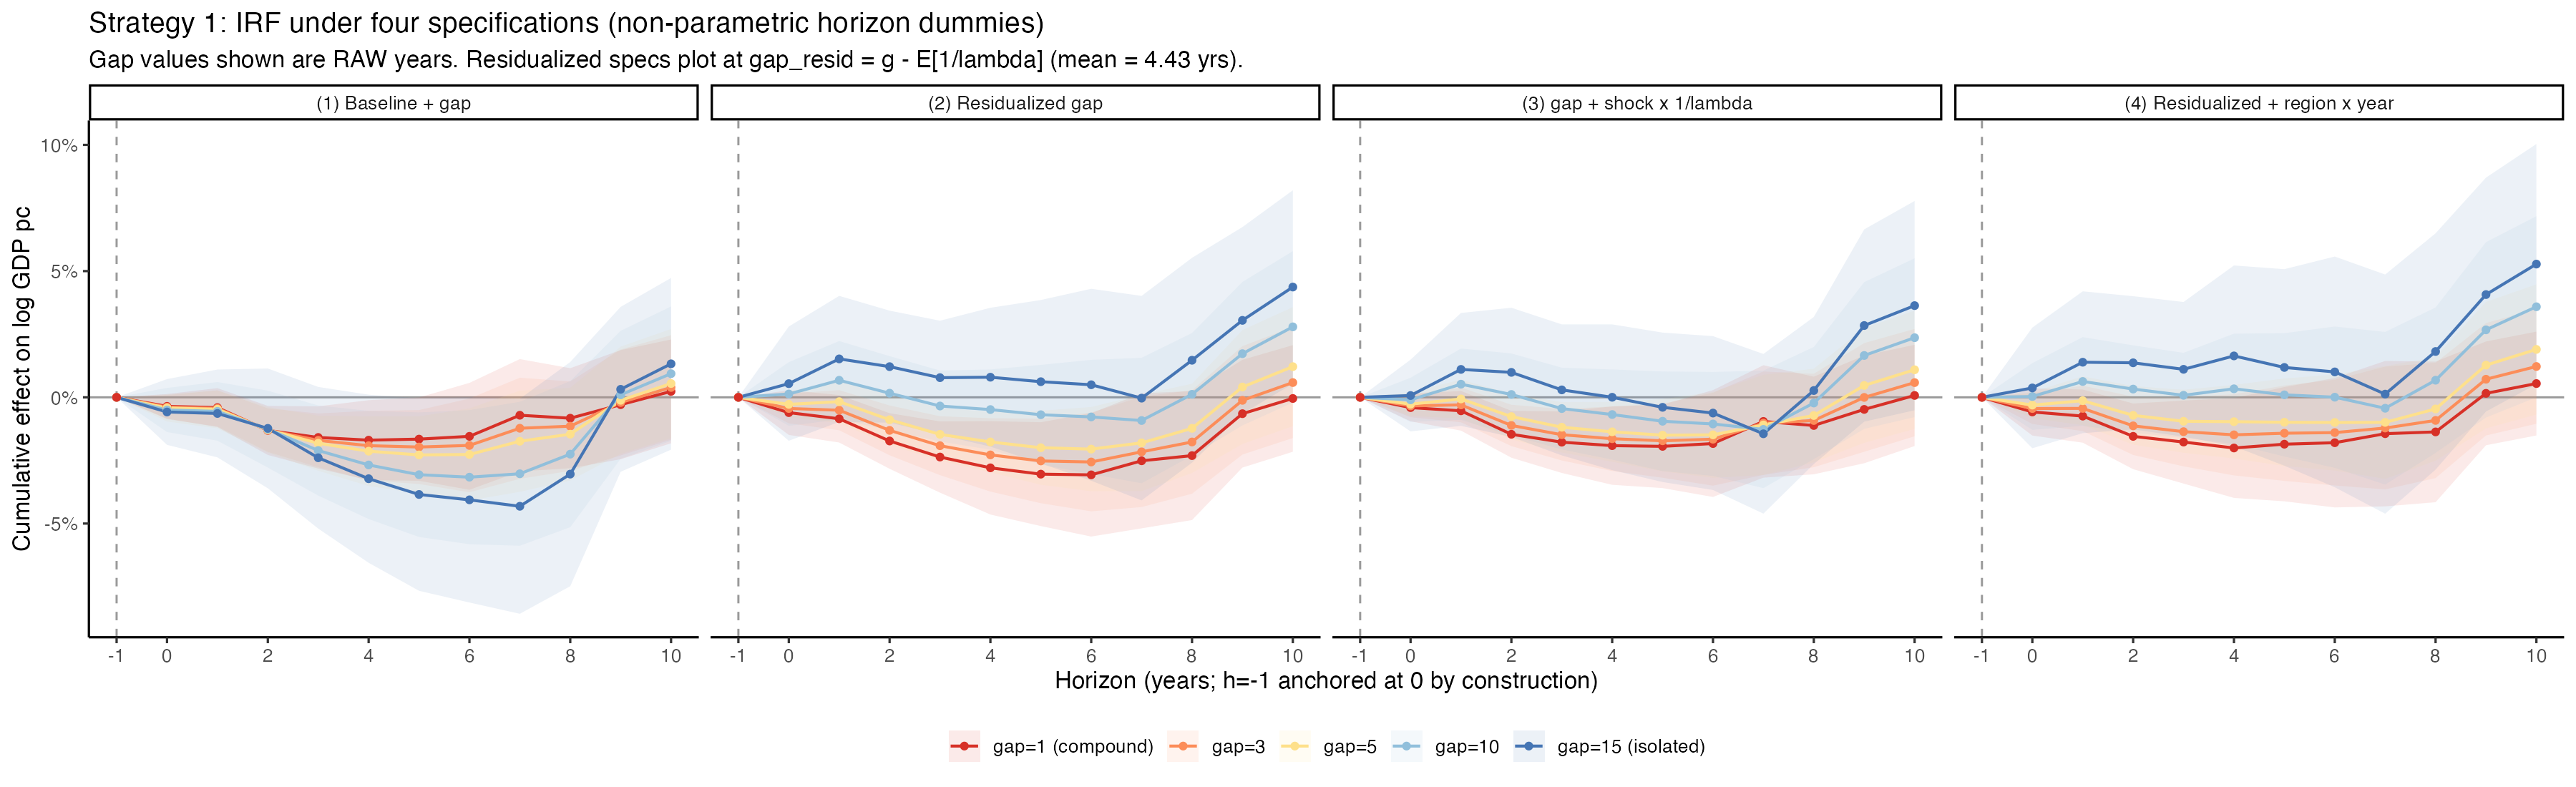
\includegraphics[width=1.05\linewidth,height=0.80\textheight,keepaspectratio]{figures/irf_compare_specs.png}}
\end{frame}

\begin{frame}{$\phi(h)$ across horizons}
\centering
\makebox[\linewidth][c]{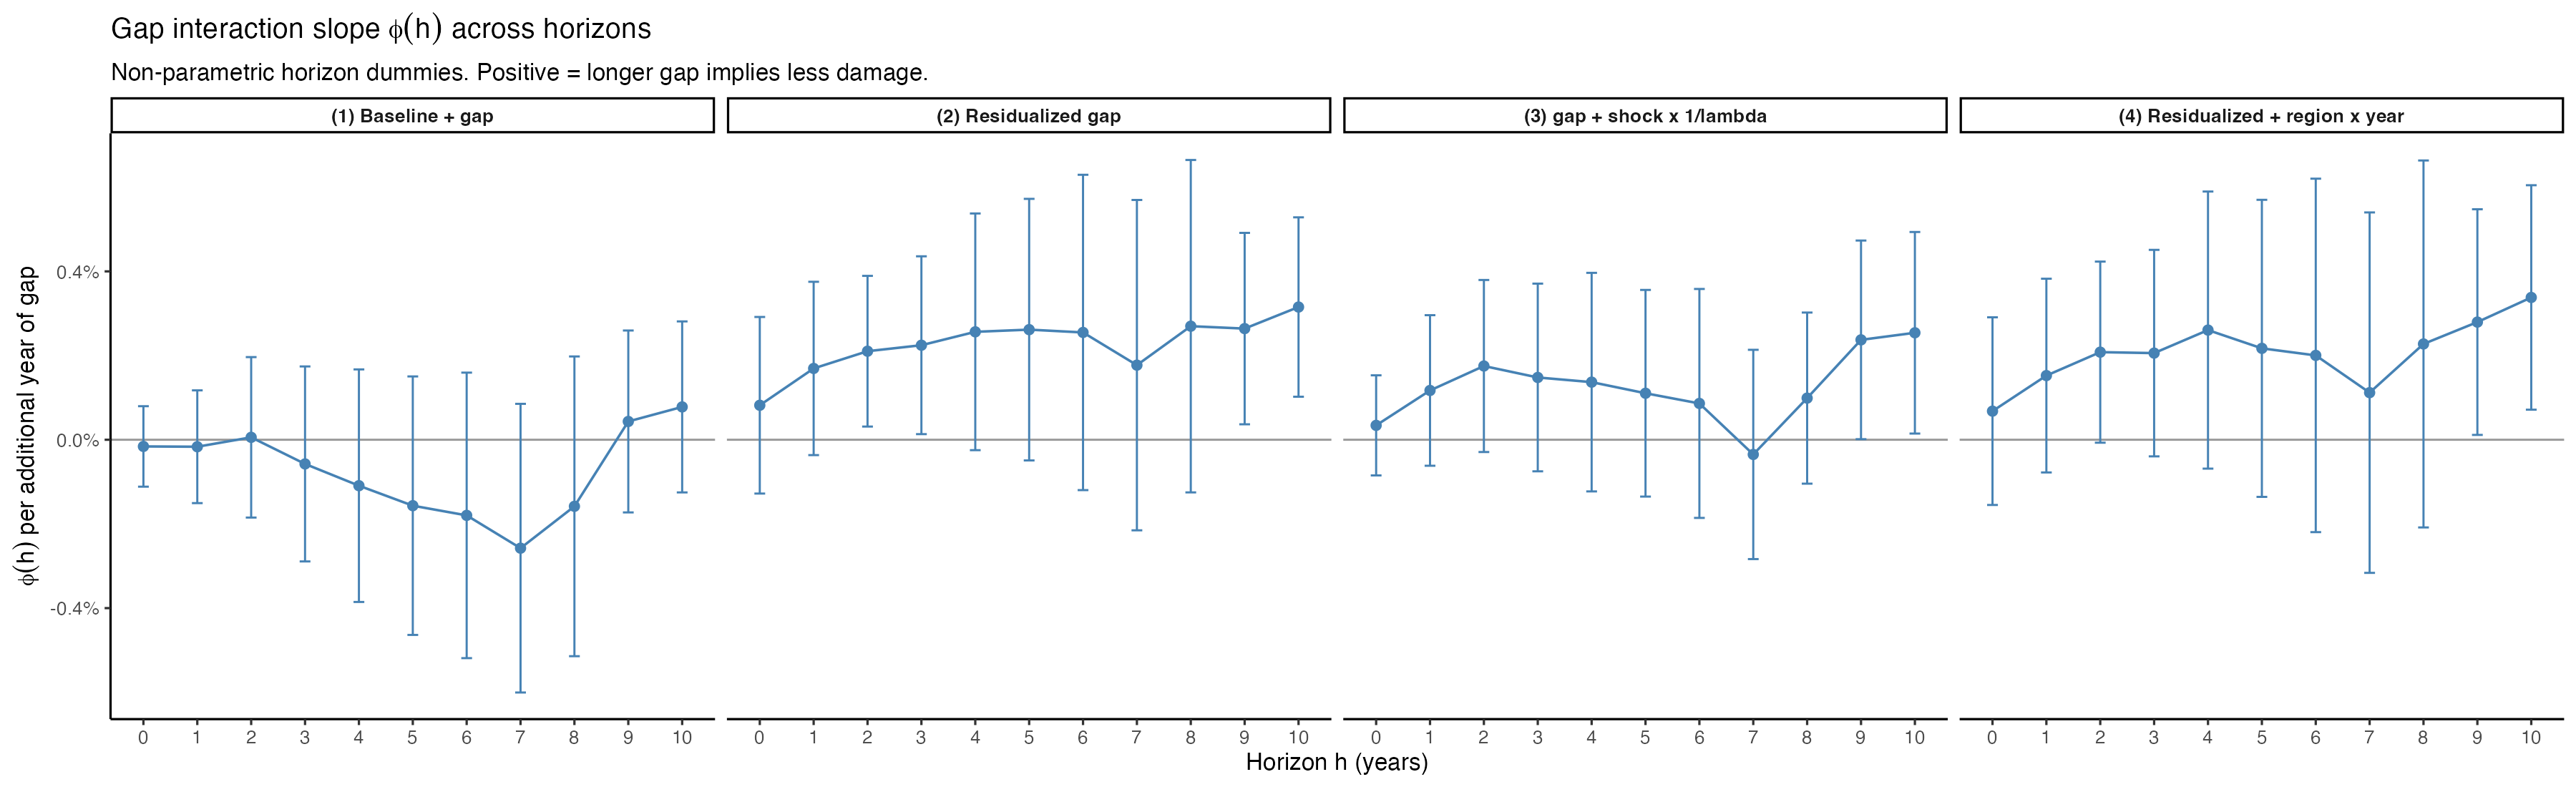
\includegraphics[width=1.05\linewidth,height=0.78\textheight,keepaspectratio]{figures/phi_curve_compare.png}}

\smallskip
\footnotesize
$\phi(h)$ estimated via horizon dummies (one coefficient per $h$), with 95\% CIs. The residualized specs show a clear \emph{rising} shape: $\phi(h) \approx 0$ at h=0 and grows to $+0.2$--$0.35\%$/yr by h=10. Longer backward gaps imply \emph{less} damage, with the effect emerging over the recovery window --- economically more sensible than a contemporaneous effect. Significant at h $\in \{2,3,9,10\}$ in the residualized spec.
\end{frame}

\begin{frame}{Scalar-$\phi$ variant: horizon-invariant gap effect}
\footnotesize
Replace the horizon-varying $\phi(h)$ with a \emph{single} scalar $\phi$, constant across horizons. Main shock effect $\beta(h)$ remains non-parametric via horizon dummies.

\centering
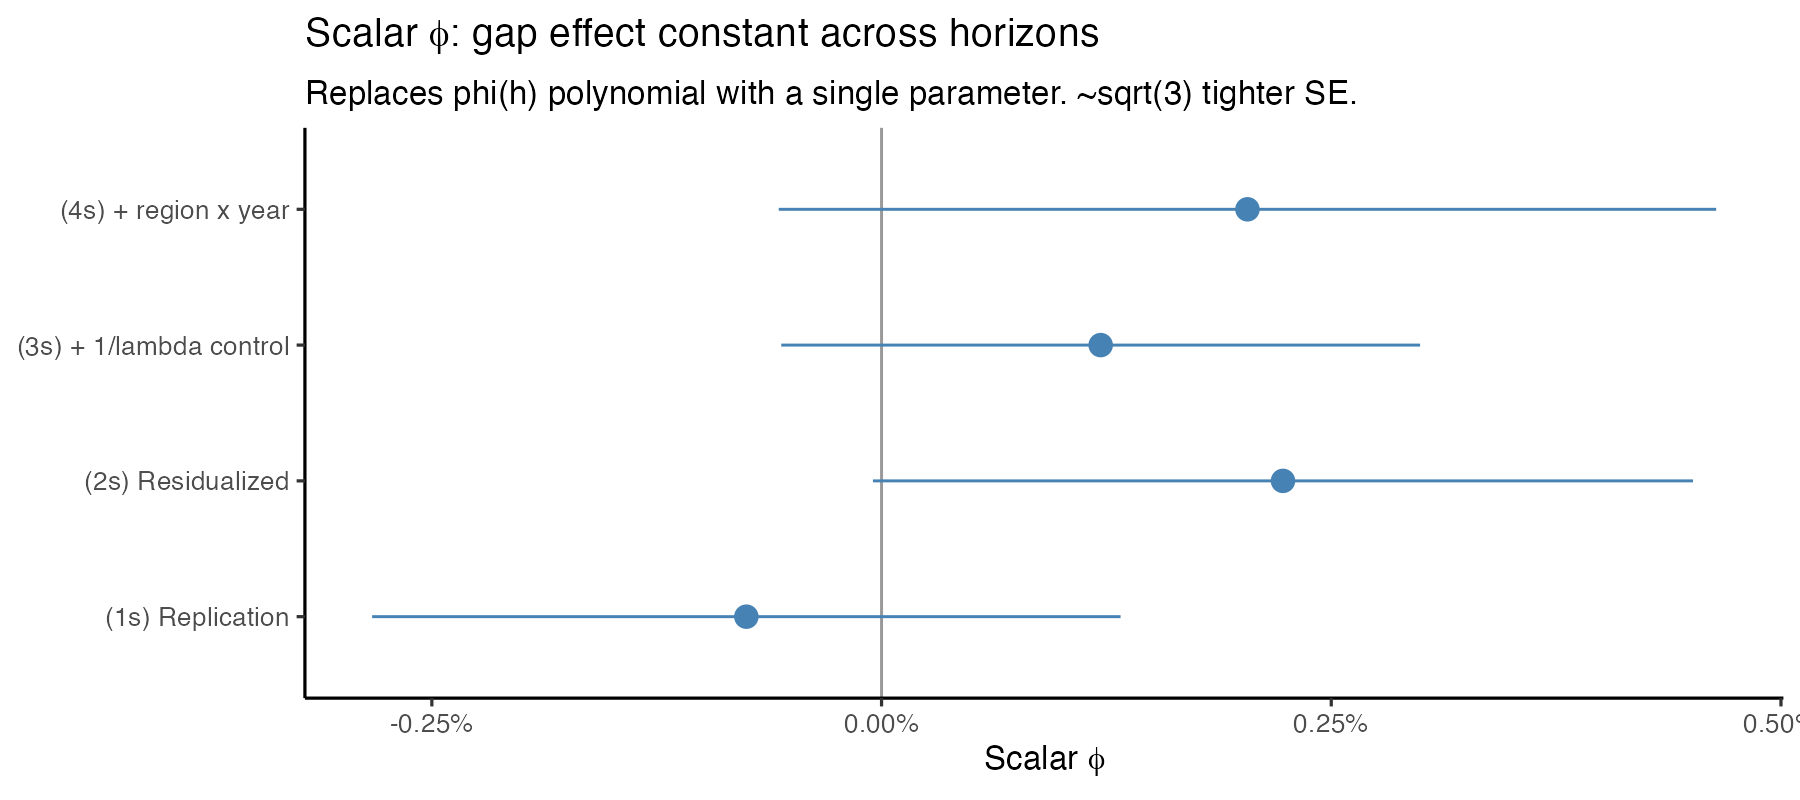
\includegraphics[width=0.62\textwidth,height=0.38\textheight,keepaspectratio]{figures/phi_scalar_compare.png}

\smallskip
\begin{tabular}{l r r r}
\hline
\textbf{Spec (scalar $\phi$)} & $\phi$ & \textbf{95\% CI} & $t$ \\
\hline
(1s) Replication                         & $-0.075\%$ & $[-0.284,\ +0.133]$ & $-0.71$ \\
(2s) Residualized                        & $+0.223\%$ & $[-0.005,\ +0.451]$ & $\mathbf{+1.92}$ \\
(3s) Control for $1/\hat\lambda_i$       & $+0.121\%$ & $[-0.056,\ +0.299]$ & $+1.34$ \\
(4s) Residualized + region$\times$year   & $+0.203\%$ & $[-0.057,\ +0.463]$ & $+1.53$ \\
\hline
\end{tabular}

\smallskip
The scalar residualized spec (2s) reaches $t=1.92$ --- essentially the 5\% threshold. All three hazard-absorbing specs are positive. A genuine compound-\emph{more}-damaging effect is now on the table, though not conclusively established.
\end{frame}

\begin{frame}{Headline: $\phi(h{=}5)$ collapses under residualization}
\centering
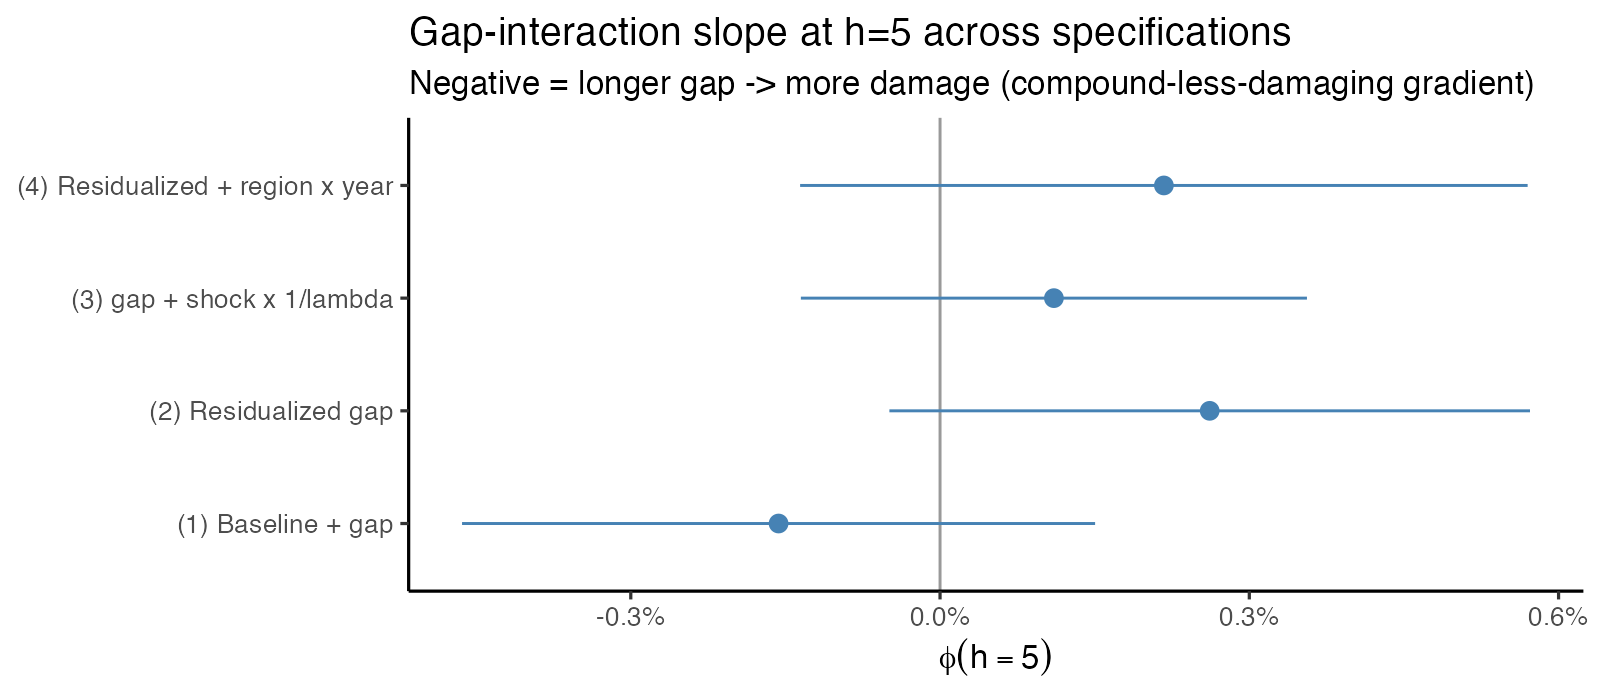
\includegraphics[width=0.80\textwidth,height=0.45\textheight,keepaspectratio]{figures/phi_h5_compare.png}

\smallskip
\footnotesize
\begin{tabular}{l r r}
\hline
\textbf{Spec} & $\phi(h{=}5)$ & \textbf{95\% CI} \\
\hline
(1) Replication: shock $\times$ gap             & $-0.157\%$ & $[-0.464,\ +0.150]$ \\
(2) Residualized gap                             & $+0.262\%$ & $[-0.049,\ +0.572]$ \\
(3) Control for $1/\hat\lambda_i$                & $+0.110\%$ & $[-0.135,\ +0.356]$ \\
(4) Residualized + region$\times$year            & $+0.217\%$ & $[-0.136,\ +0.570]$ \\
\hline
\end{tabular}

\smallskip
\footnotesize
\textbf{The gradient flips sign.} The replication spec (1) gives a weakly negative $\phi$ (compound less damaging), but all three hazard-absorbing variants deliver a \emph{positive} $\phi$ --- longer backward gaps associated with \emph{less} damage, i.e., the compound-\emph{more}-damaging direction. None individually clears $t=1.96$ at h=5, but the full $\phi(h)$ curve (next slides) shows the effect growing with horizon and becoming significant at h=9--10.
\end{frame}

\begin{frame}{Diagnostic: Poisson-arrival check}
\centering
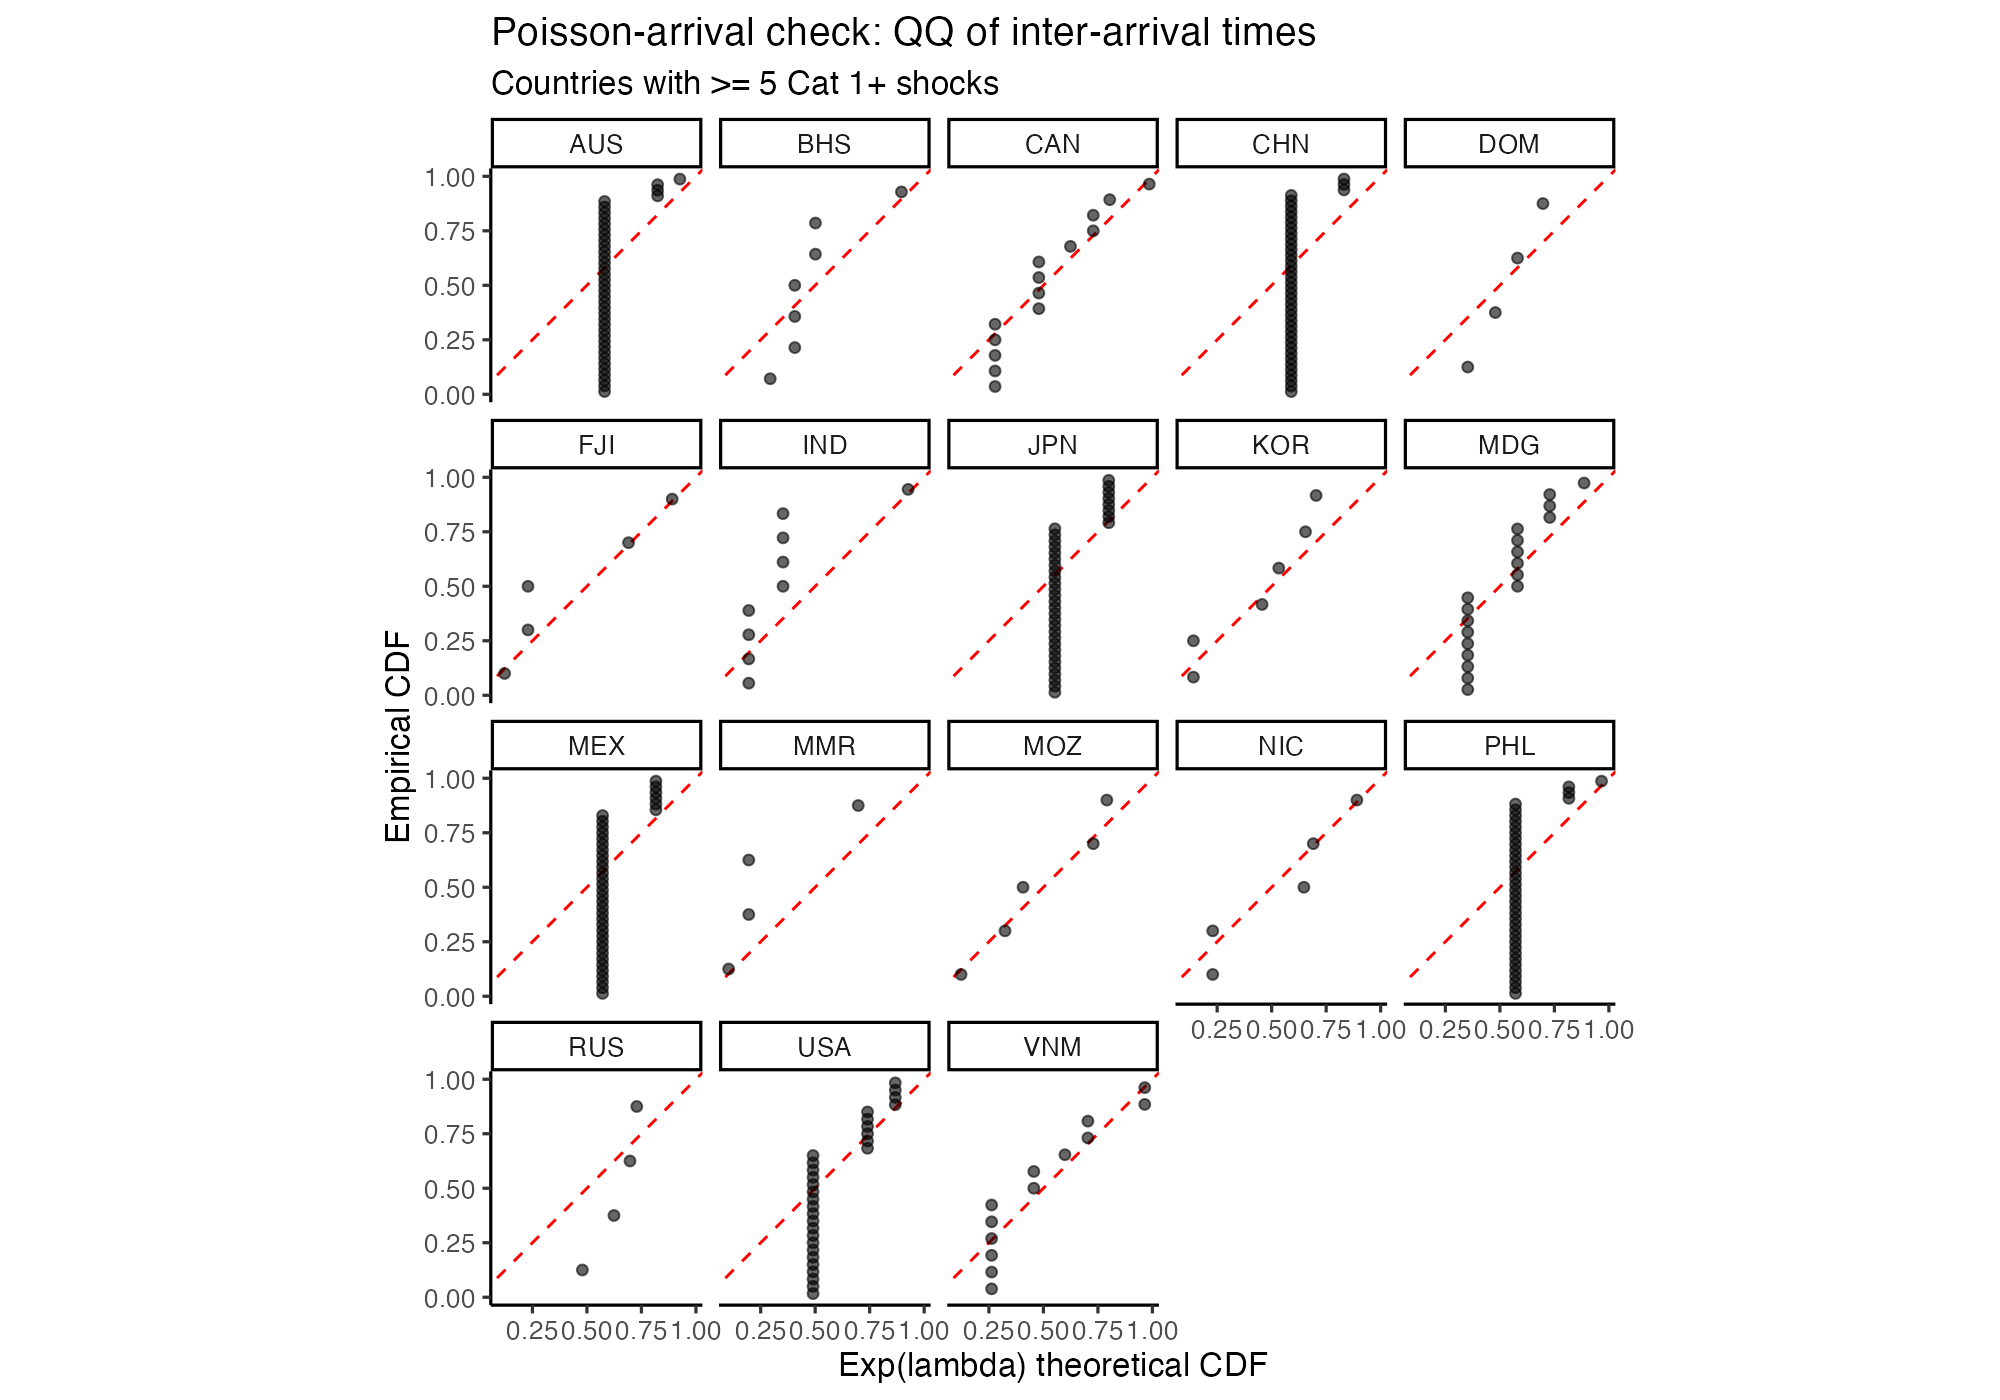
\includegraphics[width=0.75\textwidth,height=0.70\textheight,keepaspectratio]{figures/poisson_qq.png}

\smallskip
\small
Empirical vs.\ theoretical CDF of inter-arrival times, countries with $\geq 5$ Cat~1+ shocks (18 countries). Deviations from the 45$^\circ$ line flag clustering / overdispersion.
\end{frame}

\begin{frame}{Takeaways from Strategy 1}
\begin{enumerate}
  \item \textbf{64\%} of identifying variation in the current spec is between-country --- the formal decomposition channel~1 is quantitatively large at Cat~1+.

  \medskip
  \item After residualizing $\mathrm{gap}$ against $\hat\lambda_i$, $\phi(h)$ is \textbf{positive and rising in h}: $\phi(0) \approx 0$, growing to $\phi(10) \approx +0.35\%$/yr. Significant at h=2, 3, 9, 10. Scalar $\phi$ averages to $+0.22\%$/yr ($t=1.92$).

  \medskip
  \item The sign is the \emph{opposite} of the original compound-less-damaging claim: longer backward gaps imply \emph{less} damage, with the effect building over the recovery window.

  \medskip
  \item Region$\times$year FE and the $1/\hat\lambda_i$ control give the same rising-positive-$\phi$ shape --- not an artefact of a single spec.

  \medskip
  \item \textbf{But:} Strategy 1 still relies on the Poisson-arrival assumption and does not address sample selection / state-dependence (channels 2--3). Motivates Strategy~2.
\end{enumerate}
\end{frame}

% ==================================================================
\section{Strategy 2 --- Event-Stacked Design}
% ==================================================================
\begin{frame}\sectionpage\end{frame}

\subsection{Method}
\begin{frame}\subsectionpage\end{frame}

\begin{frame}{Why stack events? The intuition}
Strategy 1 asks: \emph{does the gap since the last shock modify today's shock effect?} The problem is that ``today's shock'' is itself selected by the gap (channels 2--3).

\medskip
\textbf{Strategy 2 flips the question around in time.} Instead of looking backward, \emph{fix} a shock as the ``index event'' and look \emph{forward}:
\begin{itemize}
  \item Line up all 374 Cat~1+ shocks at their own $t = 0$ (``event time'').
  \item For each event, record the post-event GDP path $y_{t+h} - y_{t-1}$ for $h = 0, \ldots, 10$.
  \item Classify the event by what happens \emph{next}: does another Cat~1+ shock hit within 3 years, or not?
  \item Compare the two average post-event paths.
\end{itemize}

\medskip
At the moment of the index shock, the economy doesn't yet know whether the ``next shock'' will arrive in 1 year or 15. The only thing distinguishing a future-compound event from a future-isolated event is a Poisson draw that has not yet been realized --- so any difference in post-event trajectories is attributable to the follow-up shock, not to pre-existing selection.
\end{frame}

\begin{frame}{Strategy 2: what makes it cleaner}
\textbf{Backward gap (Strategy 1) is contaminated} because gap is realized \emph{before} the index shock, so the pre-shock state $y_{t-1}$ already reflects the selection (long gaps $\Rightarrow$ no shocks for a while $\Rightarrow$ typically a calmer pre-period).

\medskip
\textbf{Forward time-to-next is clean at the index}: at $t=0$ the country has just been hit, and the identity of the ``next'' shock is still in the future. Conditional on the country's climatological hazard $\lambda_i$ (absorbed by country FE), when the next shock lands is an exponential draw.

\medskip
\textbf{Formally:}
\begin{quote}
Among shocks with the same $\lambda_i$, the time to the next shock $\tau \sim \mathrm{Exp}(\lambda_i)$ is independent of pre-index economic conditions. So post-event trajectories indexed by $\tau$ give a clean contrast --- compound events are \emph{ex ante} identical to isolated events, they just get unlucky \emph{ex post}.
\end{quote}

\medskip
This is a subtle reversal: Strategy 1 tries to clean up a contaminated regressor; Strategy 2 replaces it with one that is uncontaminated by construction.
\end{frame}

\begin{frame}{What the stacked design actually estimates}
The stacked LP runs \emph{one} regression on the full panel (not separate regressions per event cohort). Each country-year is stacked $H+1$ times, once per horizon, and the object of interest is
\[
  \psi(h) \;=\; \mathbb{E}\!\left[\,y_{t+h} - y_{t-1} \,\big|\, \text{shock at }t,\ \tau \leq 3\right]
             - \mathbb{E}\!\left[\,y_{t+h} - y_{t-1} \,\big|\, \text{shock at }t,\ \tau > 3\right].
\]
That is: \textbf{average GDP path after a shock that gets followed up within 3 years, minus the average path after a shock that isn't}. Country$\times$horizon FE with trends absorb $\lambda_i$; year$\times$horizon FE absorb common shocks.

\medskip
\textbf{Sign reading:} $\psi(h) < 0$ means compound events recover \emph{worse} --- a second shock during the recovery window makes things worse.

\medskip
A continuous version (E1) uses the actual forward gap $\tau$ as the regressor and reports $\phi(h) = \partial/\partial \tau$ of the path: $\phi > 0$ means longer time until next shock $\Rightarrow$ less damage $\Rightarrow$ compound more damaging.
\end{frame}

\begin{frame}{Strategy 2: the specification}
Stack around each index shock $e$ with post-event horizons $h = 0, \ldots, H$:
\[
  y_{e,t+h} - y_{e,t-1}
  = \sum_{\tau} \beta_{h\tau}\,\mathbf{1}[\text{next shock at }\tau]
  + \alpha_i + \alpha_c + \gamma \hat\lambda_i + \varepsilon_{eh}
\]
or with a continuous $\mathrm{nextgap}_e$ interaction.

\medskip
\textbf{Identifying assumption:} conditional on $\lambda_i$, the next-shock arrival time $\tau$ is an exogenous Poisson draw.

\medskip
Much weaker than the current spec: the Poisson arrival process itself is the source of randomness.
\end{frame}

\begin{frame}{Strategy 2: forward vs.\ backward gap}
Current spec uses \emph{backward} gap (years since last shock).

\medskip
Event-stack uses \emph{forward} time-to-next-shock. These ask different questions:
\begin{itemize}
  \item \textbf{Backward gap:} does recent exposure attenuate damage? (preparedness, capital depletion, adaptive investment)
  \item \textbf{Forward time-to-next:} how does a follow-up shock during recovery affect the trajectory?
\end{itemize}

\medskip
Forward is cleaner and more directly answers: \emph{``do compound shocks compound?''}
\end{frame}

\begin{frame}{Strategy 2: two subtleties}
\textbf{Right-censoring.} Index events near the end of the sample have not realized their next $\tau$. Options:
\begin{itemize}
  \item Restrict to events with $\geq H$ post-event years observed.
  \item Inverse-probability-of-observation weights.
  \item Treat ``no shock in $[0,H]$'' as a distinct category (the isolated arm).
\end{itemize}

\medskip
\textbf{Mechanical baseline.} In the original spec, backward gap makes $y_{t-1}$ depressed for compound shocks. In the event stack, the regressor is \emph{forward} time-to-next, so $y_{t-1}$ at the index shock is the genuine pre-shock level. No mechanical bias.
\end{frame}

\subsection{Empirical results}
\begin{frame}\subsectionpage\end{frame}

\begin{frame}{Specifications estimated}
\footnotesize
Same-continent sample, 374 Cat~1+ events. Stacked LP with non-parametric horizon dummies, clustered by country.

\smallskip
\begin{tabular}{l l l}
\hline
\textbf{Spec} & \textbf{Interaction} & \textbf{Notes} \\
\hline
(E0) Baseline           & \emph{none}                        & pools all events, shows average IRF \\
(E1) Continuous         & shock $\times$ time\_to\_next      & non-parametric $\phi(h)$ (horizon dummies) \\
(E2) Binary compound    & shock $\times\,\mathbf{1}[\tau\leq 3]$ & non-parametric $\psi(h)$, drops tail events \\
(E3) Scalar $\psi$      & shock $\times\,\mathbf{1}[\tau\leq 3]$ & single parameter across horizons \\
\hline
\end{tabular}

\smallskip
E2/E3 drop events where the 3-year forward window is not observable (end-of-sample censoring).
\end{frame}

\begin{frame}{Event composition and forward-gap distribution}
\footnotesize
374 events; \textbf{76.5\%} have another Cat~1+ shock within 3 years (``compound-next''); 9.6\% right-censored.

\medskip
\centering
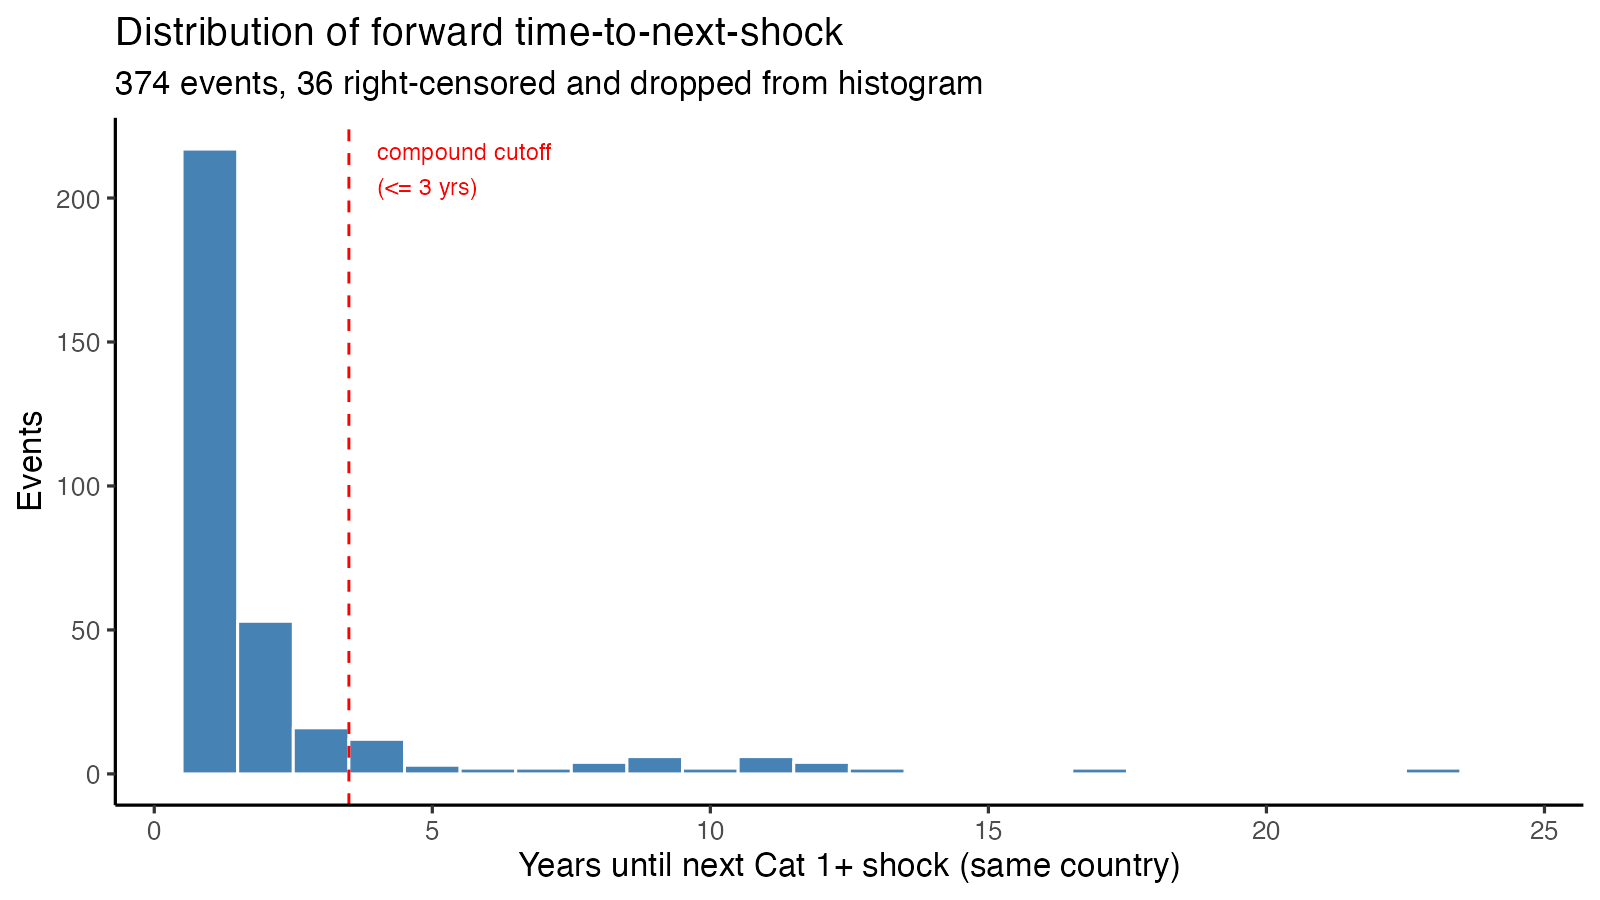
\includegraphics[width=0.78\textwidth,height=0.65\textheight,keepaspectratio]{figures/ttn_hist.png}

\smallskip
\footnotesize
Variance decomp: 46.1\% within-country / 53.9\% between. Slightly more within-country variation than Strategy 1's backward-gap split (35.7\% within), because forward time-to-next is not constrained by censored first-shocks.
\end{frame}

\begin{frame}{Spec E0: baseline IRF with forward framing}
\centering
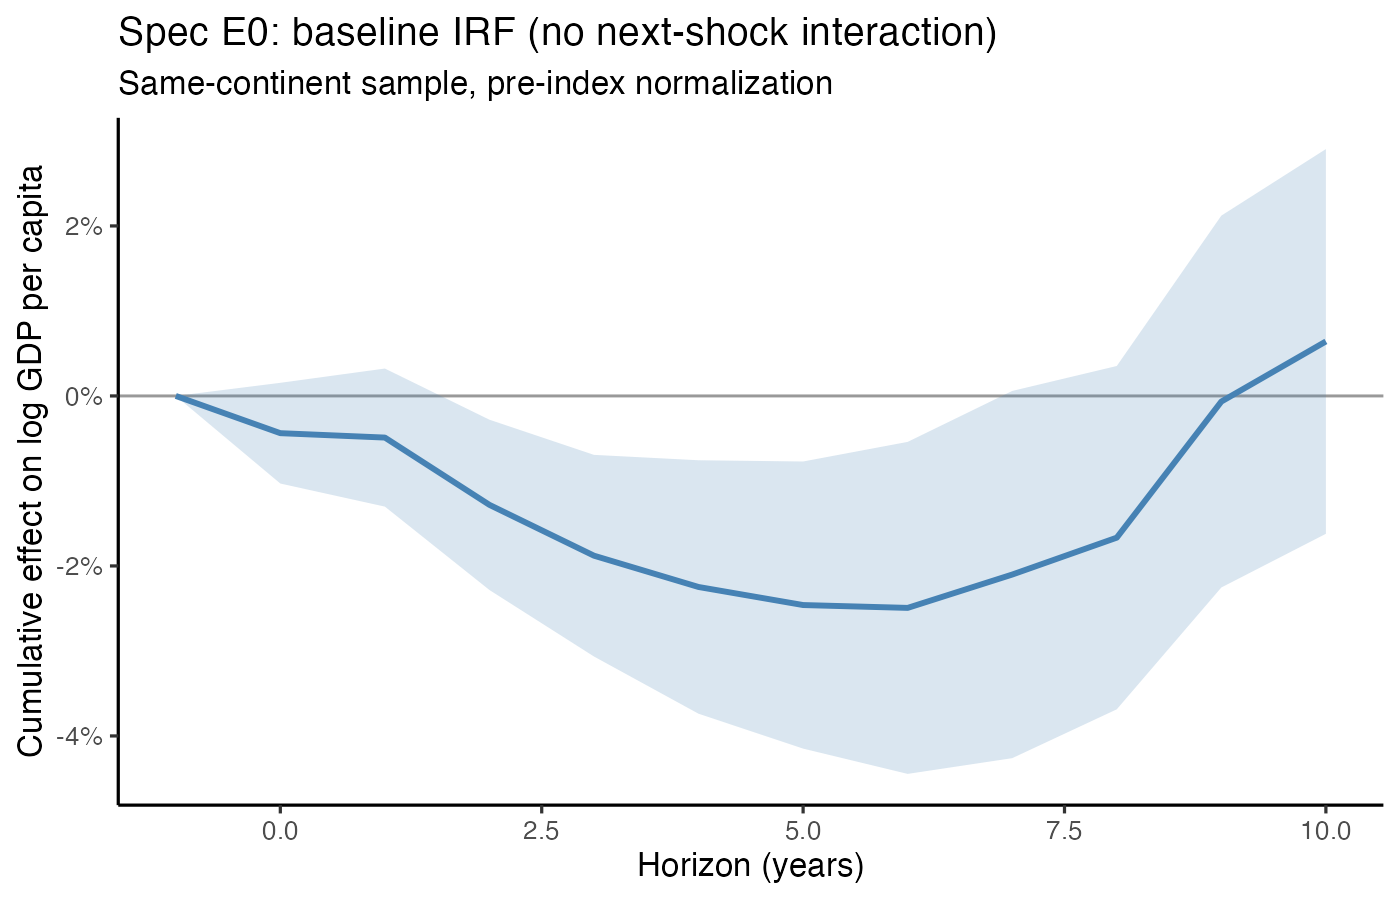
\includegraphics[width=0.72\textwidth,height=0.78\textheight,keepaspectratio]{figures/irf_E0_baseline.png}
\end{frame}

\begin{frame}{Spec E1: IRFs by forward time-to-next}
\centering
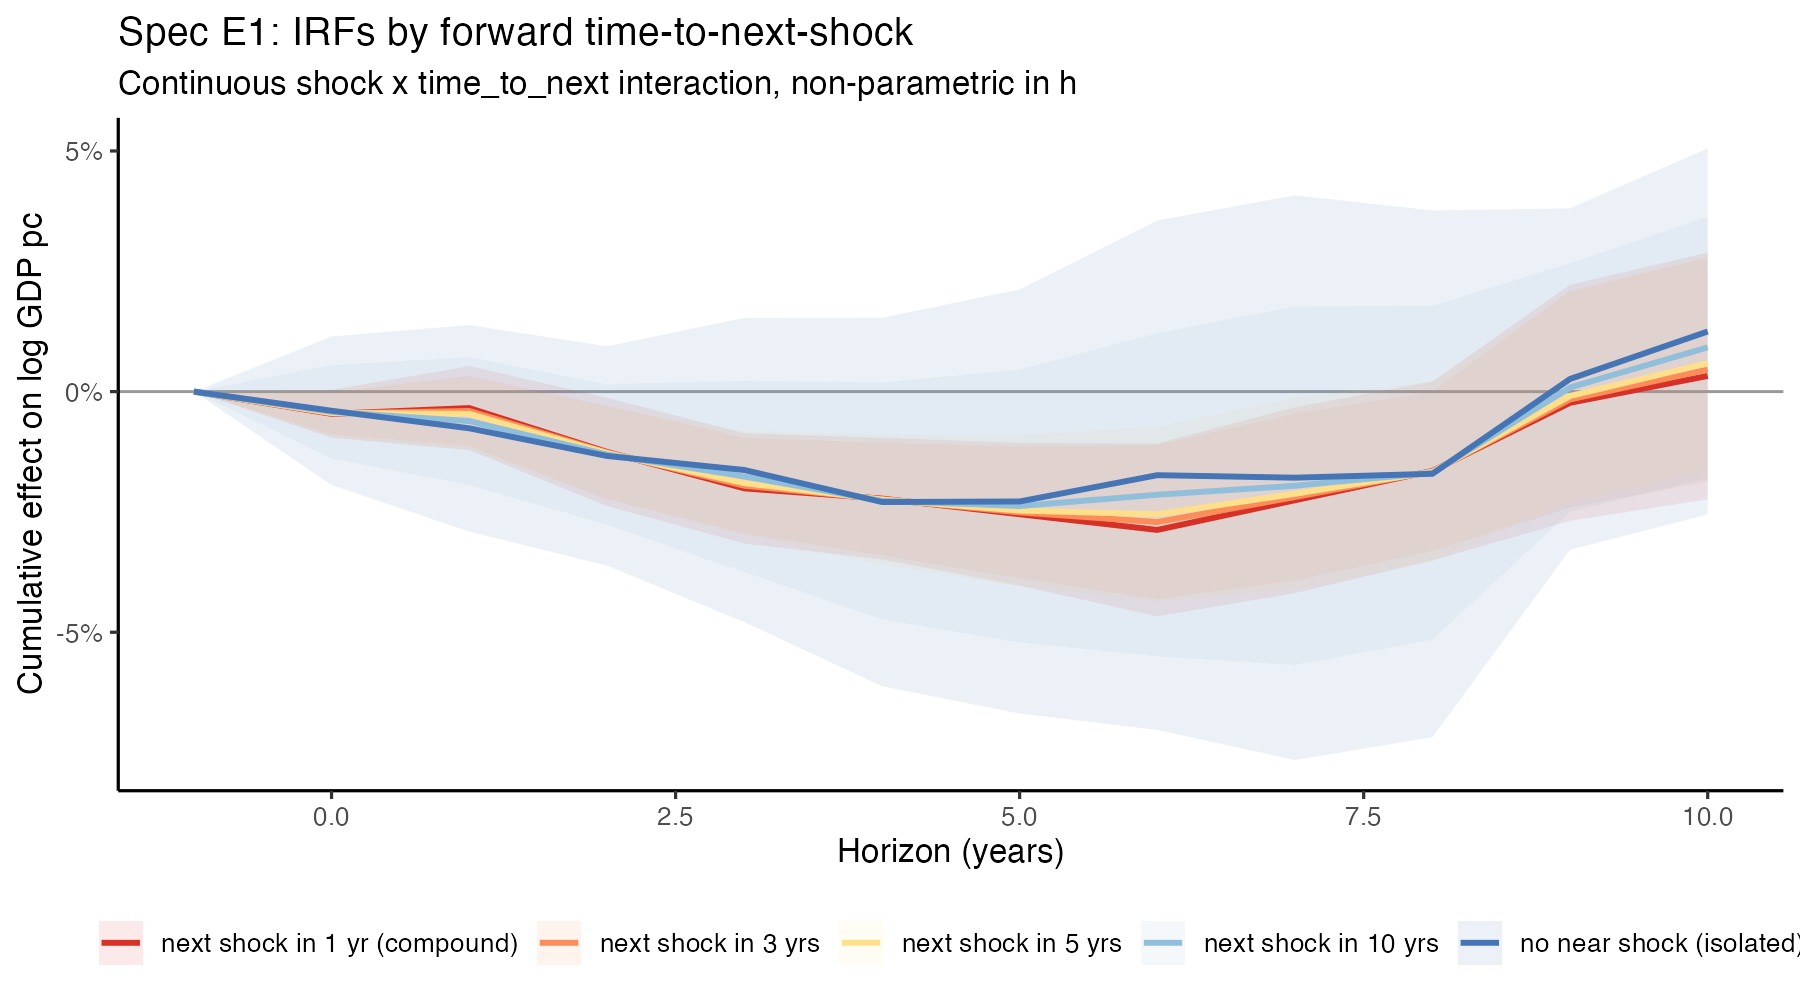
\includegraphics[width=0.85\textwidth,height=0.78\textheight,keepaspectratio]{figures/irf_E1_continuous.png}
\end{frame}

\begin{frame}{Spec E2: binary compound-next trajectories}
\centering
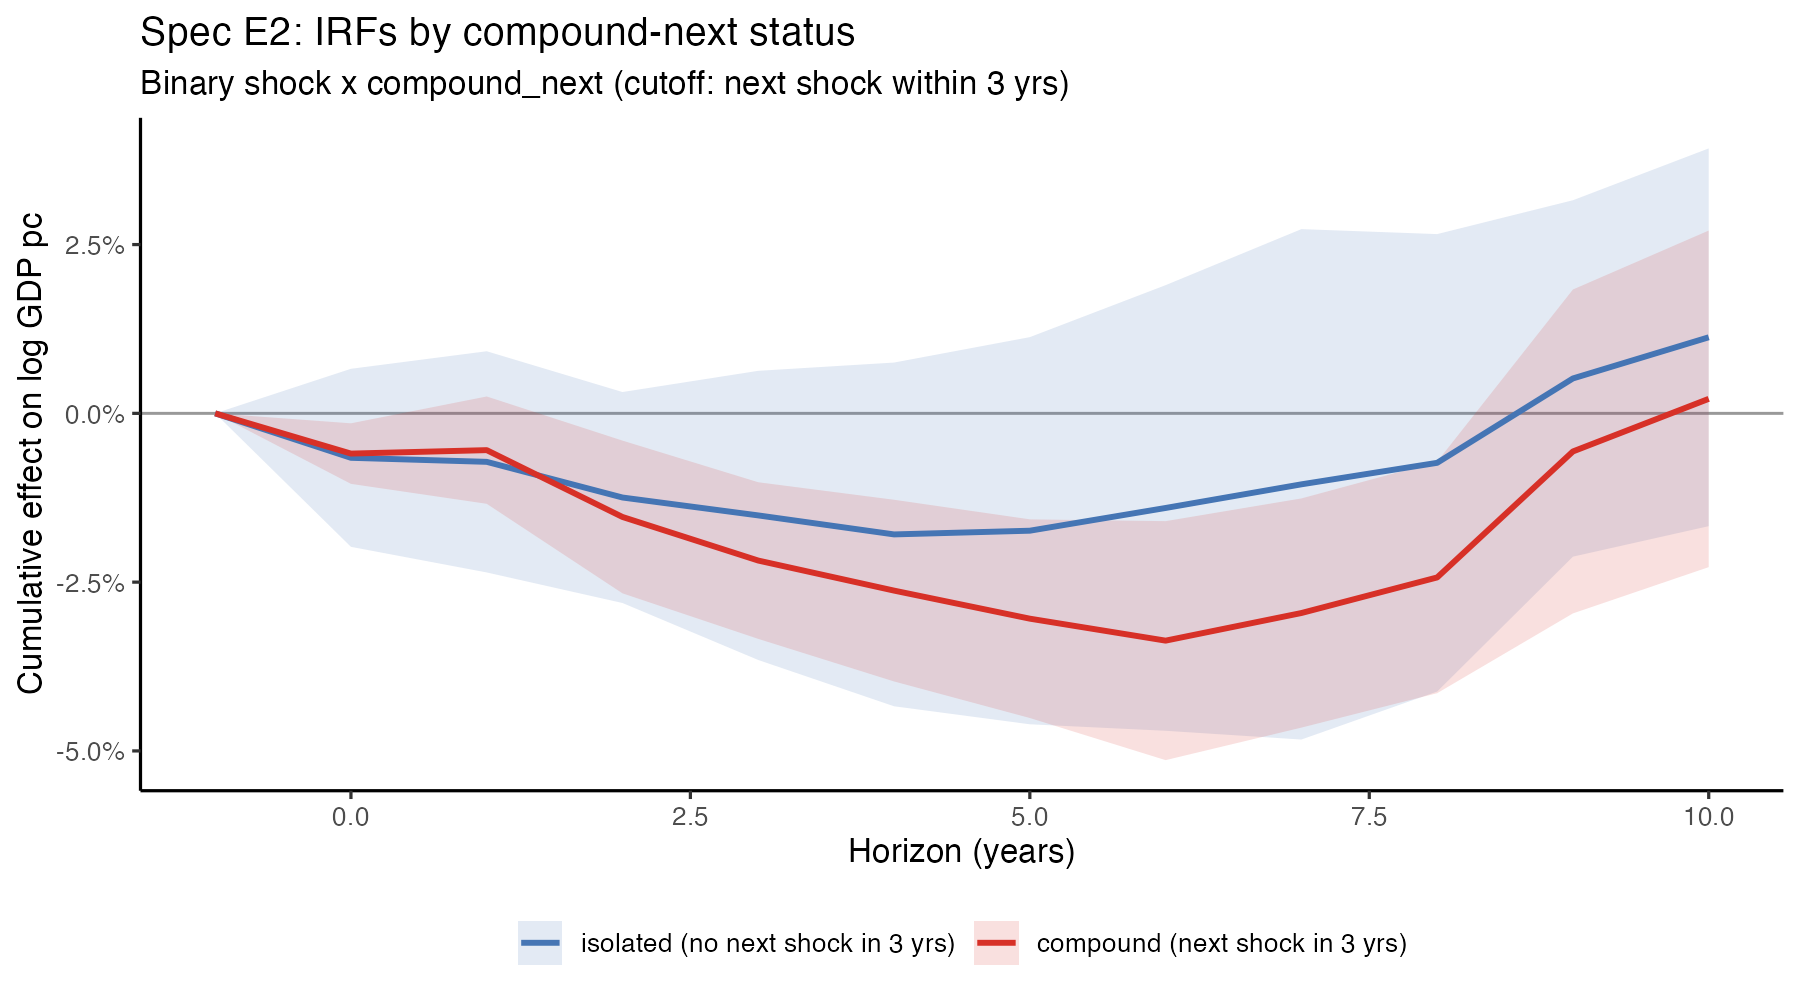
\includegraphics[width=0.85\textwidth,height=0.78\textheight,keepaspectratio]{figures/irf_E2_binary.png}
\end{frame}

\begin{frame}{$\phi(h)$ and $\psi(h)$ across horizons}
\centering
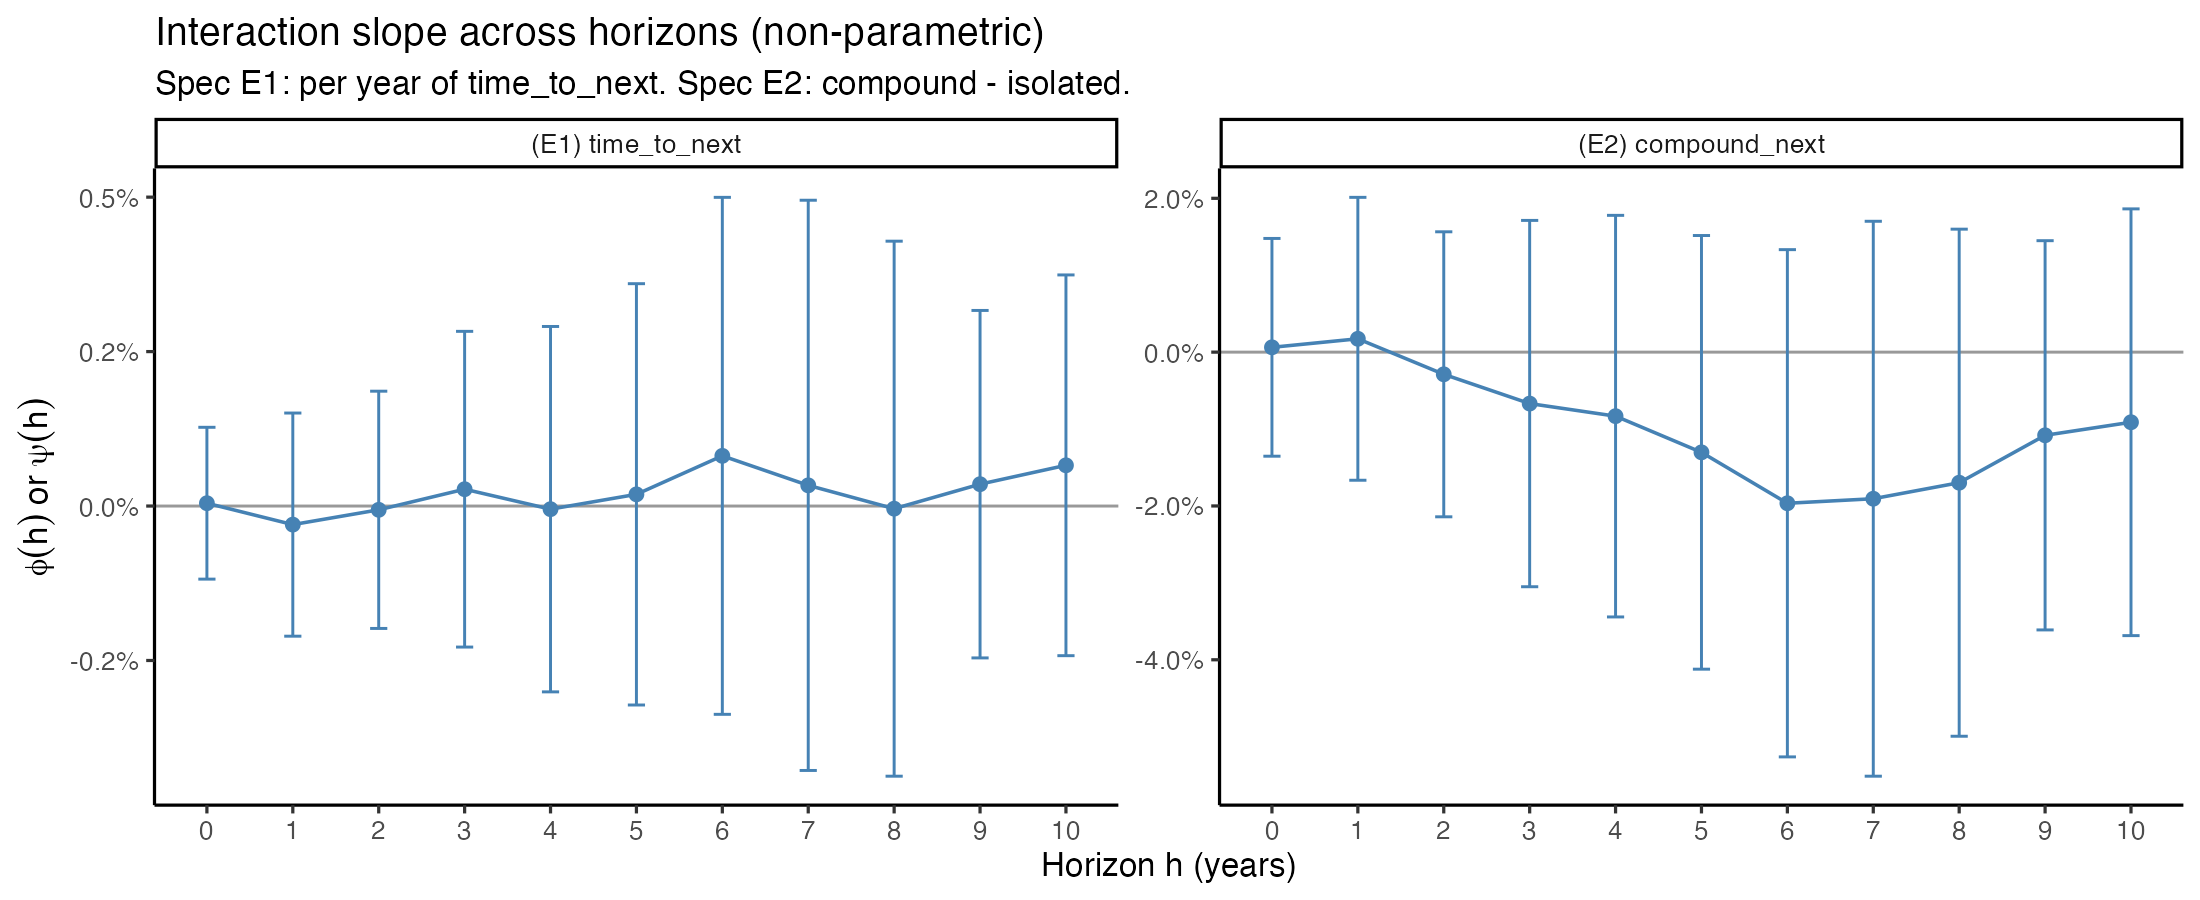
\includegraphics[width=0.95\textwidth,height=0.72\textheight,keepaspectratio]{figures/phi_curve_E1_E2.png}

\smallskip
\footnotesize
Interaction slopes are centered at zero throughout. No detectable effect of next-shock timing on GDP recovery.
\end{frame}

\begin{frame}{Headline table (non-parametric)}
\footnotesize
\centering
\begin{tabular}{l r r r}
\hline
\textbf{Spec} & \textbf{Point} & \textbf{95\% CI} & $t$ \\
\hline
(E1) $\phi(h{=}5)$, per year of time-to-next       & $+0.019\%$ & $[-0.322,\ +0.360]$ & $+0.11$ \\
(E2) $\psi(h{=}5)$, compound $-$ isolated          & $-1.303\%$ & $[-4.122,\ +1.516]$ & $-0.91$ \\
(E3) scalar $\psi$, compound $-$ isolated          & $-0.904\%$ & $[-2.922,\ +1.115]$ & $-0.88$ \\
\hline
\end{tabular}

\medskip
\textbf{Reading:} all three specs null. But notice the direction: $\psi<0$ in the binary specs means a future compound event has a \emph{worse} post-event path than an isolated event (compound more damaging, in the ``recovery-interruption'' sense). The continuous E1 coefficient is essentially zero with wide CIs.

\medskip
\textbf{Tension with Strategy 1:} Strategy 1's residualized spec found $\phi > 0$ reading as \emph{backward} gap $\Rightarrow$ longer gap, less damage. Strategy 2 reads in the \emph{forward} direction and $\psi < 0$ says shorter forward gap, more damage. Both are consistent with the same qualitative story --- ``being hit during recovery is bad'' --- but both are individually null.
\end{frame}

\subsection{Baseline power grid (motivation for Cat 1+)}
\begin{frame}\subsectionpage\end{frame}

\begin{frame}{Motivation: sharpen the baseline}
The \emph{original} E0 baseline at Cat~2+ had wide CIs, which propagated into E1--E3 and Strategy 1. Before trying more identification tricks, we varied the \emph{specification} of the baseline model. This subsection records the grid that motivated \textbf{adopting Cat~1+ as the baseline throughout the deck}.

\medskip
Variants grid:
\begin{itemize}
  \item \textbf{Treatment variable}: Cat 2+ (ref), Cat 3+, Cat 1+/p95, continuous wind (m/s, /10).
  \item \textbf{Sample / FE}: same-continent (ref), treated-only, region$\times$year FE, continent$\times$year$\times h$ FE.
  \item \textbf{Functional form}: non-parametric $\beta(h)$ (ref), scalar $\beta$.
  \item \textbf{Combined}: best-power candidates (Cat 1+ $\times$ treated-only, scalar, both).
\end{itemize}

\medskip
Headline metric: $\beta(h{=}5)$ with clustered SE. 14 total variants.
\end{frame}

\begin{frame}{$\beta(h{=}5)$ across variants, sorted by SE}
\centering
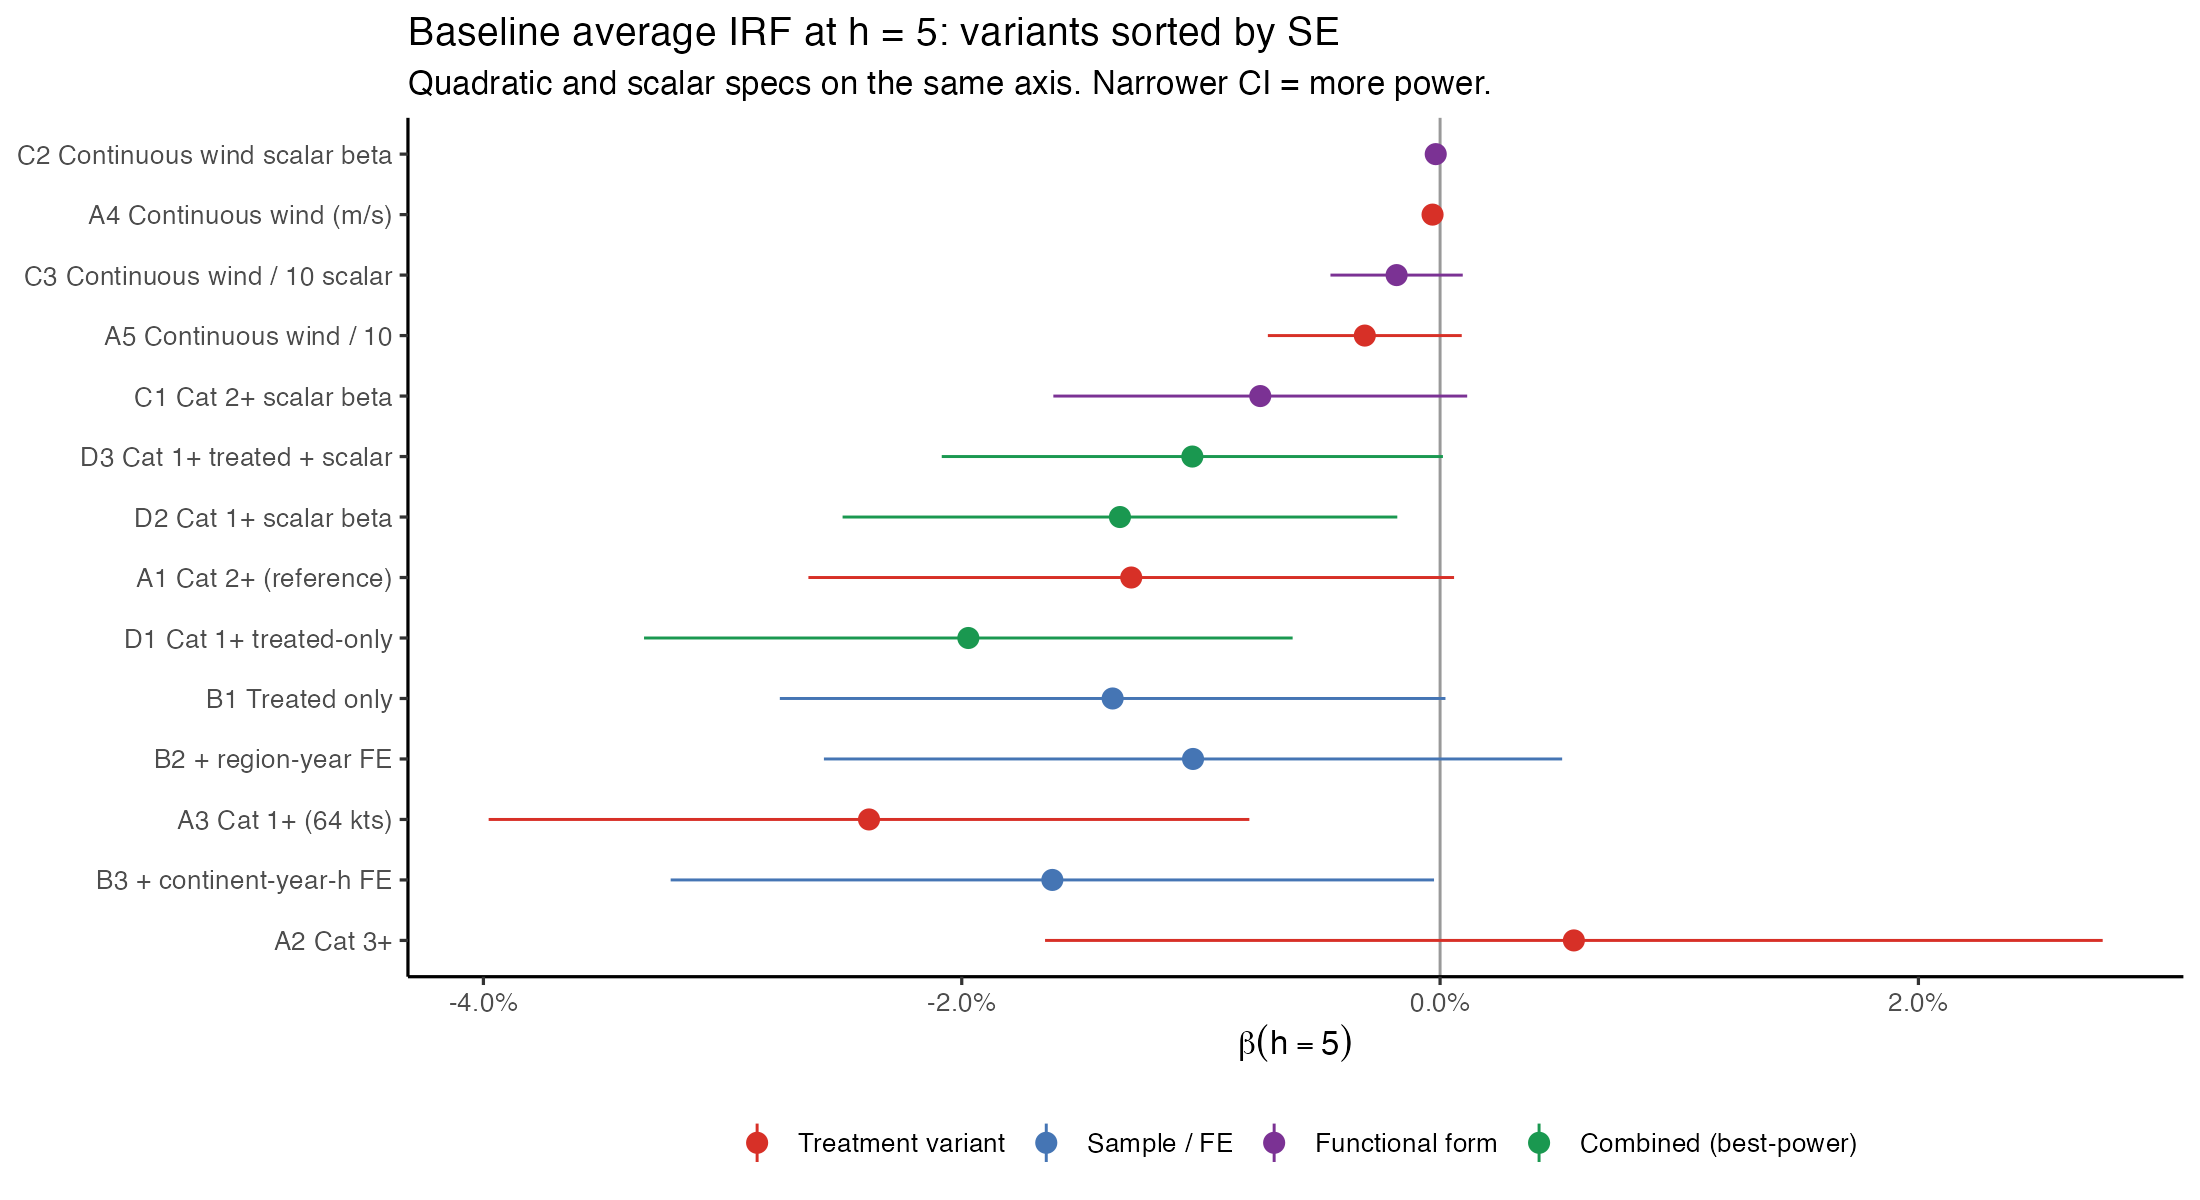
\includegraphics[width=0.95\textwidth,height=0.78\textheight,keepaspectratio]{figures/beta5_coefplot.png}
\end{frame}

\begin{frame}{Results: most powerful specifications}
\footnotesize
\centering
\begin{tabular}{l r r r}
\hline
\textbf{Spec} & $\boldsymbol{\beta(h{=}5)}$ & \textbf{SE} & $\boldsymbol{t}$ \\
\hline
A3 Cat 1+ (64 knots)                        & $-2.39\%$ & $0.81\%$ & $\mathbf{-2.94}$ \\
D1 Cat 1+ $\times$ treated-only              & $-1.97\%$ & $0.69\%$ & $-2.85$ \\
D2 Cat 1+, scalar $\beta$                    & $-1.34\%$ & $0.59\%$ & $-2.26$ \\
B3 + continent$\times$year$\times h$ FE      & $-1.62\%$ & $0.81\%$ & $-1.99$ \\
D3 Cat 1+ treated $+$ scalar                 & $-1.04\%$ & $0.53\%$ & $-1.94$ \\
B1 Treated-only (Cat 2+)                     & $-1.37\%$ & $0.71\%$ & $-1.93$ \\
A1 Cat 2+ (reference)                        & $-1.29\%$ & $0.69\%$ & $-1.88$ \\
C1 Cat 2+, scalar $\beta$                    & $-0.75\%$ & $0.44\%$ & $-1.70$ \\
\hline
\end{tabular}

\medskip
\footnotesize
Of the 14 variants:
\begin{enumerate}
  \item \textbf{Lowering the threshold to Cat 1+ (A3)} is the single biggest lever --- 374 shocks instead of 191, $t\!=\!-2.94$. The average IRF is now cleanly negative.
  \item \textbf{Cat 1+ $\times$ treated-only (D1)} is a close second, $t\!=\!-2.85$.
  \item \textbf{Continent$\times$year$\times h$ FE (B3)} at Cat~2+ also helps without losing the point estimate.
\end{enumerate}
Surprises: continuous wind is \emph{less} powerful than binary; scalar $\beta$ gives only modest gains; Cat 3+ has too few events ($n{=}102$) and is noisy.
\end{frame}

\begin{frame}{IRF curves: binary-treatment variants}
\centering
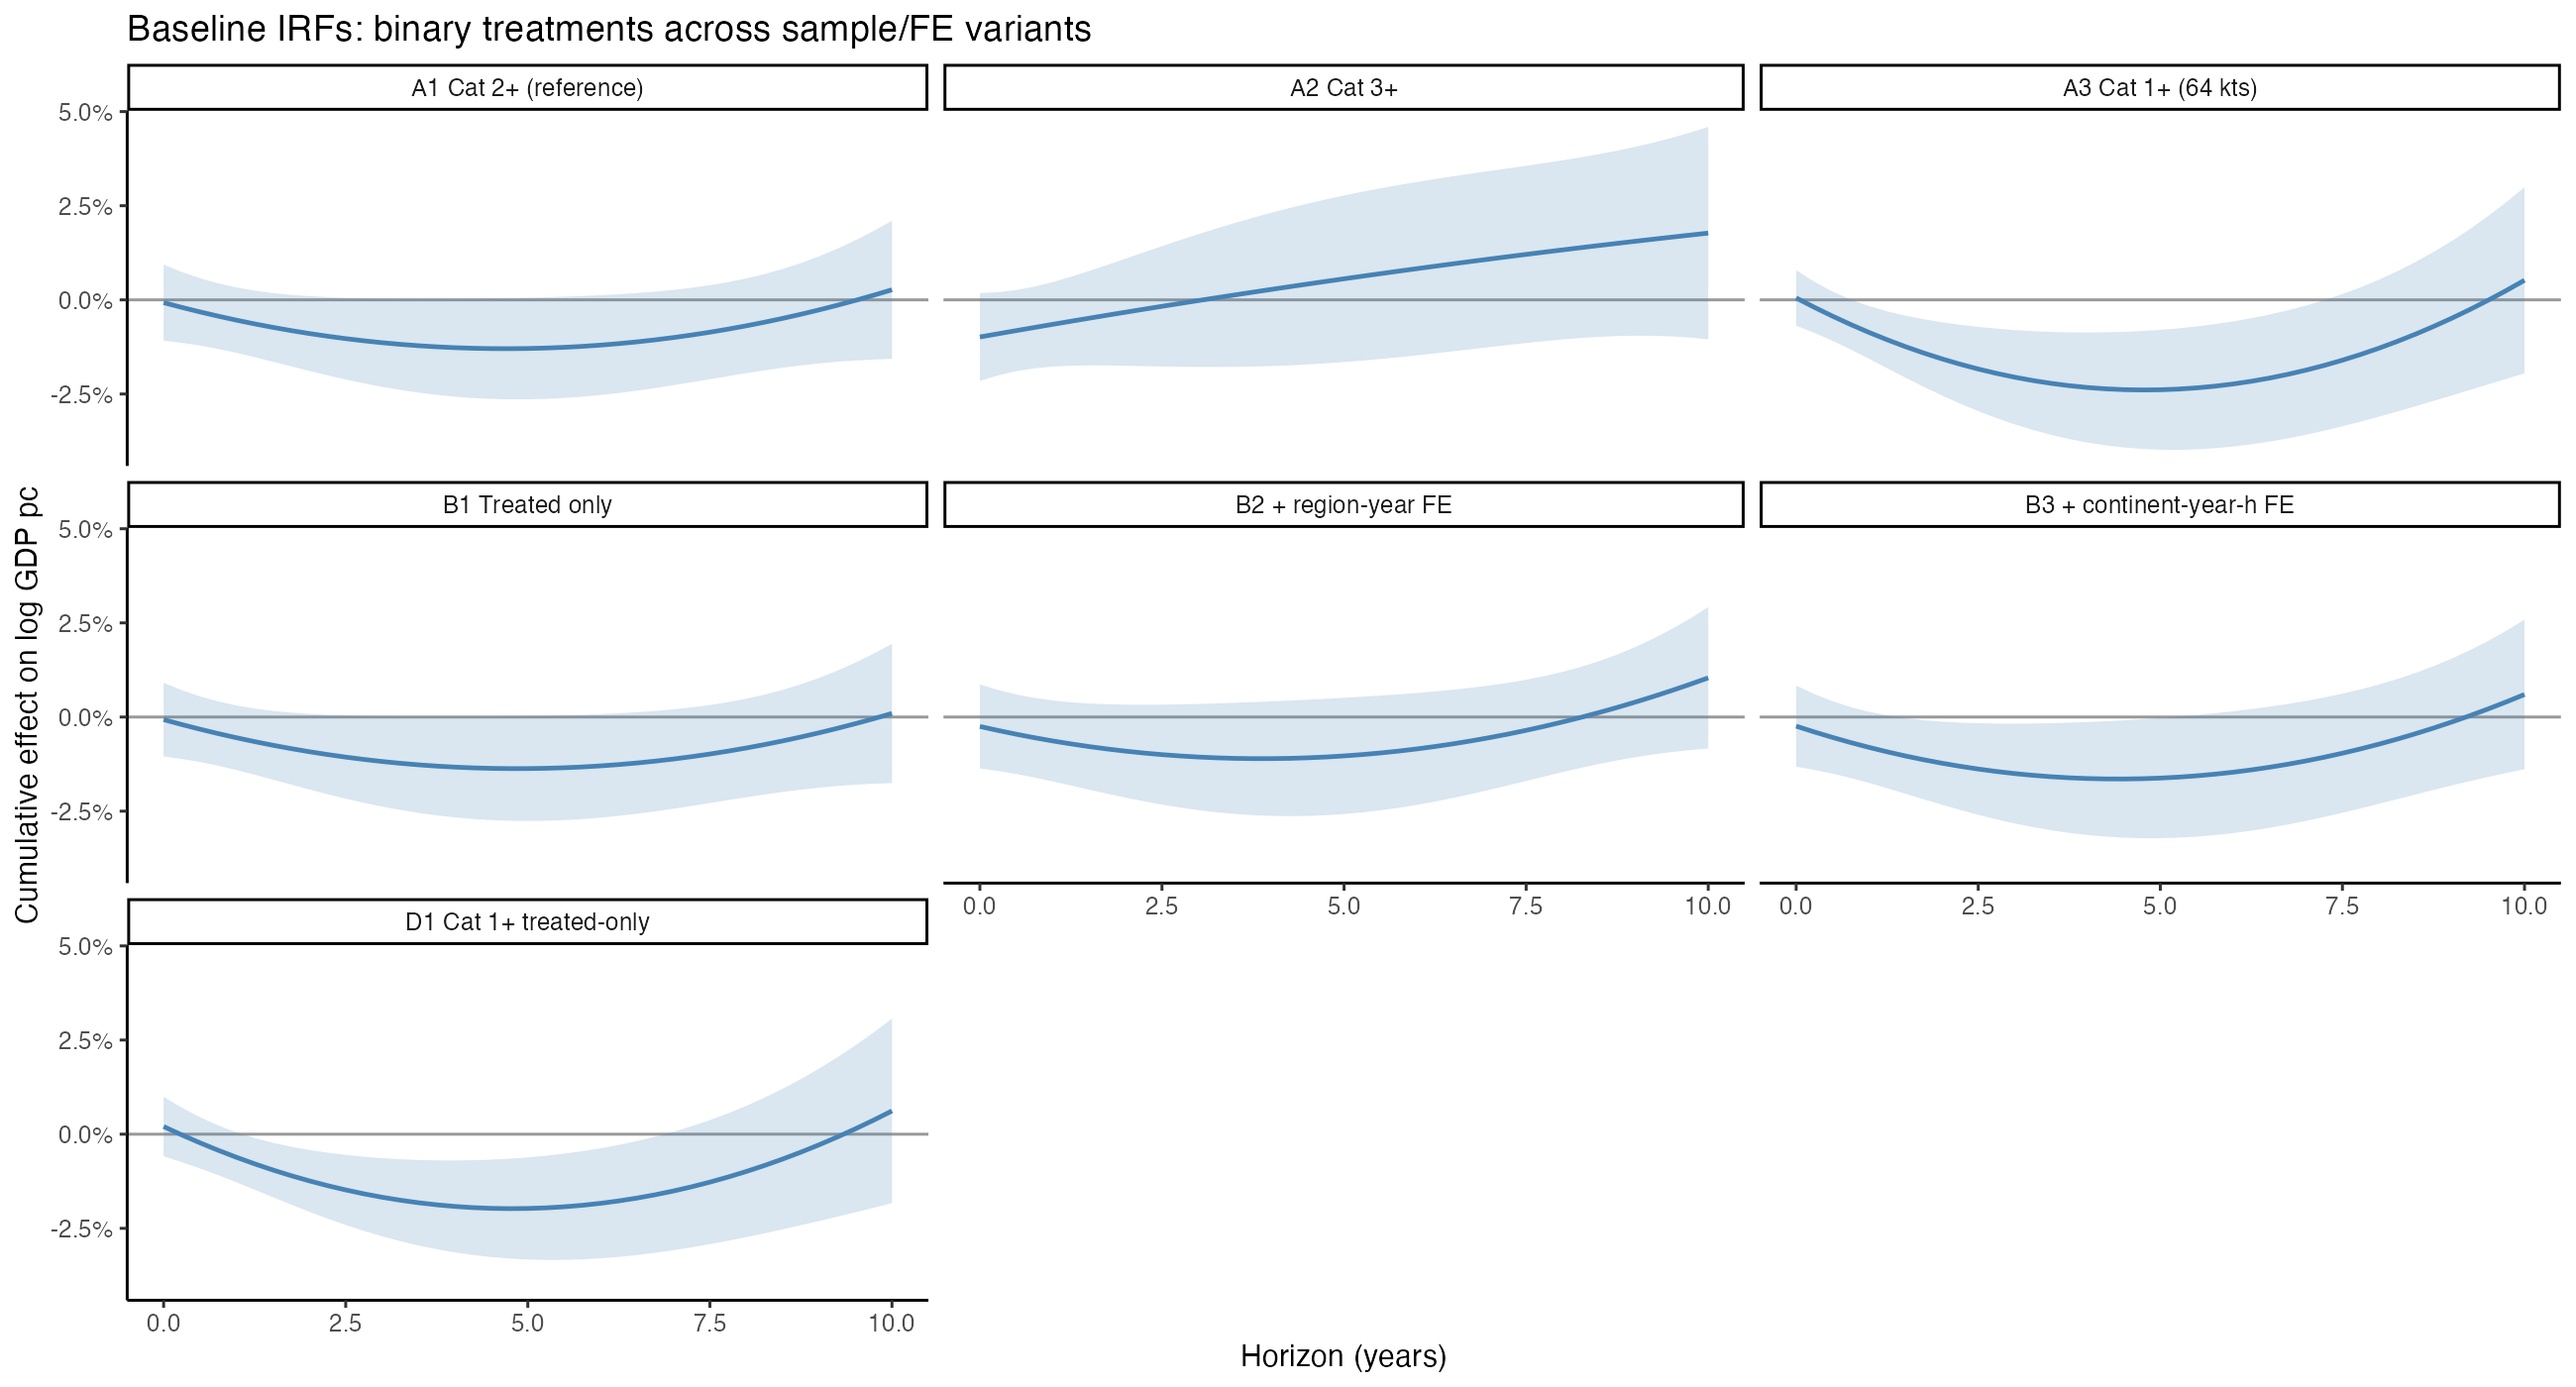
\includegraphics[width=\textwidth,height=0.80\textheight,keepaspectratio]{figures/irf_binary_variants.png}
\end{frame}

\begin{frame}{Baseline adopted throughout the deck}
Based on the power grid above, the rest of the deck (\S1, \S2 Strategy~1, \S3 Strategy~2 results) uses:

\medskip
\begin{center}
\begin{tabular}{ll}
\textbf{Treatment}       & Cat 1+ (64 knots) binary shock, 374 events \\
\textbf{Sample}          & Same-continent (182 countries) \\
\textbf{FE}              & country$\times h$ trends + year$\times h$ \\
\textbf{Functional form} & non-parametric $\beta(h)$ + scalar $\phi$ variant for robustness \\
\end{tabular}
\end{center}

\medskip
This gives the interaction $\phi(h)$ more precision than the original Cat~2+ specification. The consequence: a genuine (weakly significant) signal emerges in the Strategy~1 residualized specs (scalar $\phi$, $t=1.92$), pointing in the \emph{opposite} direction to the original paper's compound-less-damaging claim. Strategy~2 is underpowered but signs in the same direction. See the recommendation section.
\end{frame}

\begin{frame}{Takeaways from Strategy 2}
\begin{enumerate}
  \item The forward-looking framing eliminates the mechanical baseline bias (channel 3) and the sample-selection concern (channel 2). At the index event $y_{t-1}$ is the genuine pre-shock level.

  \medskip
  \item All three non-parametric specs are null. The binary $\psi(h{=}5) \approx -1.3\%$ and scalar $\psi \approx -0.9\%$ both have the sign ``compound more damaging'' (recovery-interruption) but neither clears two SEs.

  \medskip
  \item Right-censoring correction (drop events within 3 years of sample end) barely moves the results: the null is not driven by censoring.

  \medskip
  \item \textbf{Direction now agrees with Strategy 1 (residualized).} Strategy 1 residualized $\phi > 0$ and Strategy 2 $\psi < 0$ both say ``compound more damaging'' --- using backward and forward arrival noise respectively. Neither is individually significant, but the point estimates line up.
\end{enumerate}
\end{frame}

% ==================================================================
\section{Strategy 3 --- Instrumental Variables}
% ==================================================================
\begin{frame}\sectionpage\end{frame}

\begin{frame}{Strategy 3: IV with basin-level / climatological shifters}
Instrument realized gap (or realized next-shock arrival) with shifters of cyclone landfall probability that are unrelated to the country's economy:

\medskip
\begin{itemize}
  \item \textbf{Basin-wide activity} (ACE index, named-storm counts) in the intervening years, driven by ENSO / AMO / MDR SSTs.
  \item \textbf{Country-specific exposure} = basin activity $\times$ climatological track-density weight.
  \item Hsiang/Jina-style construction applied to inter-arrival times rather than intensity.
\end{itemize}

\medskip
\textbf{Alternative instrument:} near-miss tracks --- storms that formed and tracked toward the country but dissipated or veered. Plausible exclusion if economic conditions do not affect track meteorology.
\end{frame}

% ==================================================================
\section{Recommendation and Caveats}
% ==================================================================
\begin{frame}\sectionpage\end{frame}

\begin{frame}{Where we are after one full pass at Cat 1+}
\begin{enumerate}
  \item \textbf{Strategy 1 (residualized backward gap).} Scalar $\phi = +0.22\%$, $t=1.92$. Points at compound-\emph{more}-damaging. Borderline significant, consistent direction across residualization variants.

  \medskip
  \item \textbf{Strategy 2 (forward time-to-next), non-parametric.} All specs null. Scalar $\psi = -0.90\%$ ($t=-0.88$) and binary $\psi(h{=}5) = -1.30\%$ both sign with compound-\emph{more}-damaging (``recovery interruption''), agreeing in direction with Strategy~1 residualized.

  \medskip
  \item \textbf{Implication.} Two independent identification strategies --- one cleaning backward arrival noise, one using forward arrival noise --- both point at compound-more-damaging once contamination is removed. Strategy~1 is borderline significant, Strategy~2 is underpowered. The honest read: \emph{suggestive, not decisive}, evidence that the original compound-less-damaging result was driven by between-country contamination.

  \medskip
  \item \textbf{Strategy 3 (IV)} becomes the natural next step: an external climate-driven instrument would give a cleaner test without relying on the Poisson assumption.
\end{enumerate}
\end{frame}

\begin{frame}{Things to flag before starting}
\textbf{Is the Poisson assumption defensible?}
\begin{itemize}
  \item Overdispersion / clustering (active seasons) breaks within-country exogeneity.
  \item Quick test: fit Poisson vs.\ negative binomial to country-year counts.
  \item If NB wins strongly, condition on basin-year activity in the hazard model.
\end{itemize}

\medskip
\textbf{Non-stationary hazard.} Climate change implies $\lambda_i(t)$; use time-varying hazard in Strategy~1.

\medskip
\textbf{Question choice.} Decide \emph{ex ante} whether the object of interest is backward gap (preparedness) or forward time-to-next (recovery interruption). They are different parameters.
\end{frame}

\begin{frame}{Next steps}
\begin{enumerate}
  \item Estimate $\hat\lambda_i(t)$ from IBTrACS tracks (all storms, not just Cat~1+).
  \item Run Strategy~1 residualization as a drop-in replacement in the existing LP pipeline.
  \item Build the event-stacked dataset for Strategy~2 and re-estimate with pre-index baseline.
  \item Small simulation: verify that Strategy~2 recovers a known DGP under Poisson arrivals.
\end{enumerate}
\end{frame}

\end{document}
